 % cd ..\..\Users\NikitaSkybytskyi\Desktop\c3s1\complex-analysis
\documentclass[a4paper, 12pt]{article}
\usepackage[utf8]{inputenc}
\usepackage[english, ukrainian]{babel}

\usepackage{amsmath, amssymb}
\usepackage{multicol}
\usepackage{graphicx}
\usepackage{float}
\usepackage{multicol}

\usepackage{amsthm}
\newtheorem{theorem}{Теорема}[subsection]
\newtheorem*{theorem*}{Теорема}
\newtheorem{lemma}{Лема}[subsection]
\newtheorem*{lemma*}{Лема}
\newtheorem*{remark*}{Зауваження}
\theoremstyle{definition}
\newtheorem*{definition}{Визначення}
\newtheorem{problem}{Задача}[section]
\newtheorem*{solution}{Розв'язок}
\newtheorem{example}{Приклад}
\newtheorem*{example*}{Приклад}
\newtheorem*{hint}{Вказівка}

\newcommand{\Max}{\displaystyle\max\limits}
\newcommand{\Sum}{\displaystyle\sum\limits}
\newcommand{\Int}{\displaystyle\int\limits}
\newcommand{\Lim}{\displaystyle\lim\limits}

\newcommand{\RR}{\mathbb{R}}
\newcommand{\ZZ}{\mathbb{Z}}

\newcommand*\diff{\mathop{}\!\mathrm{d}}
\newcommand*\Diff[1]{\mathop{}\!\mathrm{d^#1}}

\DeclareMathOperator{\Real}{Re}
\DeclareMathOperator{\Imag}{Im}

\DeclareMathOperator{\Arg}{Arg}

\DeclareMathOperator{\Ln}{Ln}

\DeclareMathOperator{\Arctan}{Arctan}
\DeclareMathOperator{\Arcsin}{Arcsin}
\DeclareMathOperator{\Arccos}{Arccos}
\DeclareMathOperator{\Arccosh}{Arccosh}
\DeclareMathOperator{\Arctanh}{Arctanh}

\DeclareMathOperator{\arcsinh}{arcsinh}
\DeclareMathOperator{\arccosh}{arccosh}
\DeclareMathOperator{\arctanh}{arctanh}
\DeclareMathOperator{\arccoth}{arccoth}

\newcommand{\varLimsup}{\varlimsup\limits}

\makeatletter
\newcommand\xLeftrightarrow[2][]{%
  \ext@arrow 9999{\longLeftrightarrowfill@}{#1}{#2}}
\newcommand\longLeftrightarrowfill@{%
  \arrowfill@\Leftarrow\relbar\Rightarrow}
\makeatother

\renewcommand{\epsilon}{\varepsilon}
\renewcommand{\phi}{\varphi}

\allowdisplaybreaks
\setlength\parindent{0pt}
\numberwithin{equation}{subsection}

\usepackage{xcolor}
\usepackage{hyperref}
\hypersetup{unicode=true,colorlinks=true,linktoc=all,linkcolor=red}

\numberwithin{equation}{section}% reset equation counter for sections
\numberwithin{equation}{subsection}
% Omit `.0` in equation numbers for non-existent subsections.
\renewcommand*{\theequation}{%
  \ifnum\value{subsection}=0 %
    \thesection
  \else
    \thesubsection
  \fi
  .\arabic{equation}%
}


 \title{{\Huge МАТЕМАТИЧНА ФІЗИКА}}
 \author{Скибицький Нікіта}
 \date{\today}

 \usepackage{amsthm}
\usepackage[dvipsnames]{xcolor}
\usepackage{thmtools}
\usepackage[framemethod=TikZ]{mdframed}

\theoremstyle{definition}
\mdfdefinestyle{mdbluebox}{%
	roundcorner = 10pt,
	linewidth=1pt,
	skipabove=12pt,
	innerbottommargin=9pt,
	skipbelow=2pt,
	nobreak=true,
	linecolor=blue,
	backgroundcolor=TealBlue!5,
}
\declaretheoremstyle[
	headfont=\sffamily\bfseries\color{MidnightBlue},
	mdframed={style=mdbluebox},
	headpunct={\\[3pt]},
	postheadspace={0pt}
]{thmbluebox}

\mdfdefinestyle{mdredbox}{%
	linewidth=0.5pt,
	skipabove=12pt,
	frametitleaboveskip=5pt,
	frametitlebelowskip=0pt,
	skipbelow=2pt,
	frametitlefont=\bfseries,
	innertopmargin=4pt,
	innerbottommargin=8pt,
	nobreak=true,
	linecolor=RawSienna,
	backgroundcolor=Salmon!5,
}
\declaretheoremstyle[
	headfont=\bfseries\color{RawSienna},
	mdframed={style=mdredbox},
	headpunct={\\[3pt]},
	postheadspace={0pt},
]{thmredbox}

\declaretheorem[%
style=thmbluebox,name=Теорема,numberwithin=section]{theorem}
\declaretheorem[style=thmbluebox,name=Лема,sibling=theorem]{lemma}
\declaretheorem[style=thmbluebox,name=Твердження,sibling=theorem]{proposition}
\declaretheorem[style=thmbluebox,name=Наслідок,sibling=theorem]{corollary}
\declaretheorem[style=thmredbox,name=Приклад,sibling=theorem]{example}

\mdfdefinestyle{mdgreenbox}{%
	skipabove=8pt,
	linewidth=2pt,
	rightline=false,
	leftline=true,
	topline=false,
	bottomline=false,
	linecolor=ForestGreen,
	backgroundcolor=ForestGreen!5,
}
\declaretheoremstyle[
	headfont=\bfseries\sffamily\color{ForestGreen!70!black},
	bodyfont=\normalfont,
	spaceabove=2pt,
	spacebelow=1pt,
	mdframed={style=mdgreenbox},
	headpunct={ --- },
]{thmgreenbox}

\mdfdefinestyle{mdblackbox}{%
	skipabove=8pt,
	linewidth=3pt,
	rightline=false,
	leftline=true,
	topline=false,
	bottomline=false,
	linecolor=black,
	backgroundcolor=RedViolet!5!gray!5,
}
\declaretheoremstyle[
	headfont=\bfseries,
	bodyfont=\normalfont\small,
	spaceabove=0pt,
	spacebelow=0pt,
	mdframed={style=mdblackbox}
]{thmblackbox}

% \theoremstyle{theorem}
\declaretheorem[name=Запитання,sibling=theorem,style=thmblackbox]{ques}
\declaretheorem[name=Вправа,sibling=theorem,style=thmblackbox]{exercise}
\declaretheorem[name=Зауваження,sibling=theorem,style=thmgreenbox]{remark}

\theoremstyle{definition}
\newtheorem{claim}[theorem]{Твердження}
\newtheorem{definition}[theorem]{Визначення}
\newtheorem{fact}[theorem]{Факт}

\newtheorem{problem}{Задача}[section]
\renewcommand{\theproblem}{\thesection\Alph{problem}}
\newtheorem{sproblem}[problem]{Задача}
\newtheorem{dproblem}[problem]{Задача}
\renewcommand{\thesproblem}{\theproblem$^{\star}$}
\renewcommand{\thedproblem}{\theproblem$^{\dagger}$}
\newcommand{\listhack}{$\empty$\vspace{-2em}} 

 \begin{document}

 \tableofcontents

% \section{Аналіз похибок заокруглення}

\subsection{Види похибок}

Нехай необхідно розв’язати рівняння
\begin{equation}
	\label{eq:1.1}
	Au = f.
\end{equation}
За рахунок неточно заданих вхідних даних насправді ми маємо рівняння
\begin{equation}
	\label{eq:1.2}
	\tilde A \tilde u = \tilde f.
\end{equation}
Назвемо $\delta_1 = u - \tilde u$ -- \textit{неусувною похибкою}. \\

Застосування методу розв‘язання \eqref{eq:1.2} приводить до рівняння
\begin{equation}
	\label{eq:1.3}
	\tilde A_h \tilde u_h = \tilde f_h,
\end{equation}
де $h > 0$ -- малий параметр. Назвемо $\delta_2 \tilde u - \tilde u_h$ -- \textit{похибкою методу}. \\

Реалізація методу на ЕОМ приводить до рівняння
\begin{equation}
	\label{eq:1.4}
	\tilde A_h^* \tilde u_h^* = \tilde f_h^*.
\end{equation}
Назвемо $\delta_3 = \tilde u_h^* - \tilde u_h$ -- \textit{похибкою заокруглення}. \\

Тоді \textit{повна похибка} $\delta = u - \tilde u_h^* = \delta_1 + \delta_2 + \delta_3$. \\

\begin{definition}
	Кажуть, що задача \eqref{eq:1.1} \textit{коректна}, якщо
	\begin{enumerate}
		\item $\forall f \in F$ $\exists! u \in U$;
		\item задача \eqref{eq:1.1} \textit{стійка}, тобто
		\begin{equation}
			\label{eq:1.5}
			\forall \epsilon > 0 \quad \exists \delta > 0: \|A-\tilde A\| < \delta, \|f-\tilde f\| < \delta \Rightarrow \|u - \tilde u\| < \epsilon.
		\end{equation}
	\end{enumerate}
\end{definition}

Якщо задача \eqref{eq:1.1} \textit{некоректна}, то або розв‘язок її не існує, або він неєдиний, або він нестійкий, тобто 
\begin{equation}
	\label{eq:1.6}
	\exists \epsilon > 0: \forall \delta > 0: \exists A, f: \| A - \tilde A\|<\delta, \|f-\tilde f\| < \delta, \|u-\tilde u\| > \epsilon.
\end{equation}

\textit{Абсолютна похибка} $\Delta (x^*) \ge \max_x |x - x^*|$. \\

\textit{Відносна похибка} $\delta (x^*) \ge \max_x \Delta (x^*) / |x^*|$. \\

\textit{Значущими цифрами} називаються всі цифри, починаючи з першої ненульової зліва. \\

\textit{Вірна цифра} -- це значуща, якщо абсолютна похибка за рахунок відкидання всіх молодших розрядів не перевищує одиниці розряду цієї цифри. Тобто, якщо 
\begin{equation}
	\label{eq:1.7}
	x^* = \overline{\alpha_n \ldots \alpha_0.\alpha_{-1}\ldots\alpha_{-p}\ldots},
\end{equation}
то $\alpha_{-p}$ -- вірна, якщо $\Delta (x^*) \le 10^{-p}$. \\

Інколи $\Delta (x^*) \le w \cdot 10^{-p}$, $1/2 \le w < 1$, наприклад, $w = 0.55$.

\subsection{Підрахунок похибок в ЕОМ}

Підрахуємо відносну похибку заокруглення числа $x$ на ЕОМ з плаваючою комою. В $\beta$-ічній системі числення число представляється у вигляді
\begin{equation}
	\label{eq:1.8}
	x = \pm (\alpha_1 \beta^{-1} + \alpha_2 \beta^{-2} + \ldots + \alpha_t \beta^{-t} + \ldots) \beta^p,
\end{equation}
де $0 \le \alpha_k < \beta$, $\alpha_1 \ne 0$, $k = 1,2,\ldots$ \\

Якщо в ЕОМ $t$ розрядів, то при відкиданні молодших розрядів ми оперуємо з наближеним значенням 
\begin{equation}
	\label{eq:1.9}
	x^* = \pm (\alpha_1 \beta^{-1} + \alpha_2 \beta^{-2} + \ldots + \alpha_t \beta^{-t}) \beta^p,
\end{equation}
і відповідно похибка заокруглення 
\begin{equation}
	\label{eq:1.9_1}
	x - x^* = \pm \beta^p (\alpha_{t+1} \beta^{-t-1} + \ldots)
\end{equation}
Тоді її можна оцінити так
\begin{multline}
	\label{eq:1.10}
	|x - x^*| \le \beta^{p-t-1} \cdot (\beta-1) \cdot (1 + \beta^{-1}+\ldots)\le\\
	\le \beta^{p-t-1} \cdot (\beta-1) \cdot \dfrac{1}{1-\beta^{-1}}=\beta^{p-t}.
\end{multline}

Якщо в представлені \eqref{eq:1.8} взяти $\alpha_1 = 1$, то $|x| \ge \beta^p \cdot \beta^{-1}$. Звідси остаточно 
\begin{equation}
	\label{eq:1.11}
	\delta (x^*) \le \dfrac{\beta^{p-t}}{\beta^{p-1}}=\beta^{1-t}.
\end{equation}

При більш точних способах заокруглення можна отримати оцінку $\delta (x^*) \le \beta^{1-t} / 2 = \epsilon$. Число $\epsilon$ називається ``машинним іпсилон''. Наприклад, для $\beta = 2$, $t = 24$, $\epsilon = 2^{-24} \approx 10^{-7}$.

\subsection{Підрахунок похибок обчислення значення функції}

Нехай задана функція 
\begin{equation}
	\label{eq:1.11_1}
	y = f(x_1, \ldots, x_n) \in C^1(\Omega)
\end{equation}
Необхідно обчислити її значення при наближеному значенні аргументів 
\begin{equation}
	\label{eq:1.11_2}
	\vec x^* = (x_1^*, \ldots, x_n^*),
\end{equation}
де $|x_i - x_i^*| \le \Delta (x_i^*)$ та оцінити похибку обчислення значення функції
\begin{equation}
	\label{eq:1.11_3}
	y^* = f(x_1^*, \ldots, x_n^*).
\end{equation}

Маємо 
\begin{equation}
	\label{eq:1.12}
	|y-y^*| = |f\left(\vec x\right) - f\left(\vec x^*\right)| = \left| \Sum_{i=1}^n \dfrac{\partial f}{\partial x_i} \left(\vec \xi\right) (x_i - x_i^*) \right| \le \Sum_{i=1}^n B_i \cdot \Delta (x_i^*), 
\end{equation}
де 
\begin{equation}
	\label{eq:1.13}
	B_i = \Max_{\vec x \in U} \left| \dfrac{\partial f}{\partial x_i}\left(\vec x\right) \right|.
\end{equation}

Тут 
\begin{equation}
	\label{eq:1.14}
	U = \left\{ \vec x = (x_1, \ldots, x_n): |x_i - x_i^*| \le \Delta (x_i^*)\right\} \in \Omega, \quad i=\overline{1,n}.
\end{equation}
Отже
\begin{equation}
	\label{eq:1.15}
	\Delta (y^*) = |y - y^*| \prec \Sum_{i=1}^n n_i \cdot \Delta (x_i^*),
\end{equation}
з точністю до величин першого порядку малості по
\begin{equation}
	\label{eq:1.15_1}
	\Delta (x^*) = \Max_{i=\overline{1,n}} \Delta (x_i^*),
\end{equation}
де
\begin{equation}
	\label{eq:1.16}
	b_i = \left| \dfrac{\partial f}{\partial x_i}\left(\vec x^*\right) \right|
\end{equation}
та ``$\prec$'' означає приблизно менше. \\

\subsubsection{Похибки арифметичних операцій}

\begin{enumerate}
	\item Сума: $y = x_1 + x_2$, $x_1, x_2 > 0$, 
	\begin{equation}
		\label{eq:1.17}
		\begin{aligned}
		\Delta (y^*) &\le \Delta (x_1^*) + \Delta (x_2^*), \\ 
		\delta (y^*) &\le \dfrac{\Delta (x_1^*) + \Delta (x_2^*)}{x_1^* + x_2^*} \le \max\{\delta (x_1^*), \delta (x_2^*)\}.
		\end{aligned}
	\end{equation}
	
	\item Різниця: $y = x_1 - x_2$, $x_1 > x_2 > 0$,
	\begin{equation}
		\label{eq:1.18}
		\begin{aligned}
		\Delta (y^*) &\le \Delta (x_1^*) + \Delta (x_2^*), \\
		\delta (y^*) &\le \dfrac{x_2^* \delta (x_1^*) + (x_1^*) \delta (x_2^*)}{x_1^* - x_2^*}.
		\end{aligned}
	\end{equation}
	
	При близьких $x_1^*$, $x_2^*$ зростає відносна похибка (за рахунок втрати вірних цифр).

	\item Добуток: $y = x_1 \cdot x_2$, $x_1, x_2 > 0$,
	\begin{equation}
		\label{eq:1.19}
		\begin{aligned}
		\Delta (y^*) &\prec x_2^* \Delta (x_1^*) + x_1^* \Delta (x_2^*), \\
		\delta (y^*) &\le \delta (x_1^*) + \delta (x_2^*).
		\end{aligned}
	\end{equation}

	\item Частка: $y = \dfrac{x_1}{x_2}$, $x_1, x_2 > 0$,
	\begin{equation}
		\label{eq:1.20}
		\begin{aligned}
		\Delta (y^*) &\prec \dfrac{x_2^* \Delta (x_1^*) + x_1^* \Delta (x_2^*)}{(x_2^*)^2}, \\
		\delta (y^*) &\le \delta (x_1^*) + \delta (x_2^*).
		\end{aligned}
	\end{equation}

	При малих $x_2^*$ зростає абсолютна похибка (за рахунок зростання результату ділення). 
\end{enumerate}

\subsection{Обернена задача аналізу позибок}

Нагадаємо, що \textit{пряма задача} аналізу похибок полягає у обчисленні $\Delta (y^*), \delta (y^*)$ по заданих $\Delta (x_i^*)$, $i = \overline{1, n}$. \\

\textit{Обернена задача} полягає у знаходженні $\Delta (x_i^*)$, $i = \overline{1, n}$ по заданих $\Delta (y^*)$, $\delta (y^*)$. Якщо $n > 1$, маємо одну умову 
\begin{equation}
	\label{eq:1.21}
	\Sum_{i=1}^n b_i \Delta (x_i^*) < \epsilon
\end{equation}
для багатьох невідомих $\Delta (x_i^*)$. Вибирають їх із однієї з умов 
\begin{equation}
	\label{eq:1.22}
	b_i \Delta (x_i^*) < \dfrac{\epsilon}{n},
\end{equation}
або
\begin{equation}
	\label{eq:1.23}
	\Delta (x_i^*) < \dfrac{\epsilon}{\Sum_{i=1}^n b_i}.
\end{equation}
% \section{Нелінійні рівняння}

\textit{Постановка задачі}. Нехай маємо рівняння $f(x) = 0$, $\overline{x}$ -- його розв’язок, тобто $f (\overline{x}) \equiv 0$. \\

Задача розв‘язання цього рівняння розпадається на етапи:
\begin{enumerate}
	\item Існування та кількість коренів.
	\item Відділення коренів, тобто розбиття числової вісі на інтервали, де знаходиться один корінь.
	\item Обчислення кореня із заданою точністю $\epsilon$.
\end{enumerate}

Для розв'язання перших двох задач використовуються методи математичного аналізу та алгебри, а також графічний метод. Далі розглядаються методи розв'язання третього етапу.

\subsection{Метод ділення навпіл}

Припустимо на $[a, b]$ знаходиться лише один корінь рівняння 
\begin{equation}
	\label{eq:2.1}
	f(x) = 0,
\end{equation}
для $f(x) \in C([a,b])$, який необхідно визначити. Нехай $f(a) \cdot f (b) < 0$. \\

Припустимо, що $f(a) > 0$, $f(b) < 0$. Покладемо $x_1 = \frac{a + b}{2}$ і підрахуємо
$f(x_1)$. Якщо $f_1(x) < 0$, тоді шуканий корінь $x$ знаходиться на інтервалі $(a, x_1)$. Якщо ж $f_1(x) > 0$, то $\overline{x} \in (x_1, b)$, тобто з двох інтервалів $(a, x_1)$ і $(x_1, b)$ вибираємо той, на границях якого функція $f(x)$ має різні знаки, знаходимо точку $x_2$ -- середину вибраного інтервалу, підраховуємо $f(x_2)$ і повторюємо вказаний процес. \\

В результаті отримаємо послідовність інтервалів, що містять шуканий корінь $\overline{x}$, причому довжина кожного послідуючого інтервалу вдвічі менше попереднього. \\

Цей процес продовжується до тих пір, поки довжина отриманого інтервалу $(a_n, b_n)$ не стане меншою за $b_n - a_n < 2 \epsilon$. Тоді $x_{n+1}$, як середина інтервалу $(a_n, b_n)$ пов'язане з $\overline{x}$ нерівністю
\begin{equation}
	\label{eq:2.2}
	|x_n+1 - \overline{x}| < \epsilon.
\end{equation}

Ця умова для деякого $n$ буде виконуватись за теоремою Больцано-Коші. \\

Оскільки
\[ |b_{k + 1} - a_{k + 1} | = \dfrac12 |b_k - a_k|, \]
то
\begin{equation}
	\label{eq:2.3}
	|x_{n+1} - \overline{x}| \le \dfrac{1}{2^{n+1}} (b - a) < \epsilon.
\end{equation}

Звідси отримаємо нерівність для обчислення кількості ітерацій $n$ для виконання умови (\ref{eq:2.2}):
\[ n = n(\epsilon) \ge \left\lfloor \log\left(\dfrac{b-a}{\epsilon}\right) \right\rfloor + 1. \]

Степінь збіжності -- лінійна, тобто геометричної прогресії з знаменником $q = \frac12$. \\

Переваги методу: простота, надійність. Недоліки методу: низька швидкість збіжності; метод не узагальнюється на системи. 

\subsection{Метод простої ітерації}

Спочатку рівняння
\begin{equation}
	\label{eq:2.4}
	f (x) = 0
\end{equation}
замінюється еквівалентним
\begin{equation}
	\label{eq:2.5}
	x = \phi(x)
\end{equation}
Ітераційний процес має вигляді
\begin{equation}
	\label{eq:2.6}
	x_{n+1} = \phi(x_n), \quad n = 0,1,\ldots
\end{equation}

Початкове наближення $x_0$ задається. \\

Для збіжності велике значення має вибір функції $\phi(x)$. Перший спосіб заміни рівняння полягає в відділенні змінної з якогось члена рівняння. Більш продуктивним є перехід від рівняння (\ref{eq:2.4}) до (\ref{eq:2.5}) з функцією $\phi (x) = x + \tau (x) \cdot f (x)$, де $\tau (x)$ -- знакостала функція на тому відрізку, де шукаємо корінь. \\

Кажуть, що ітераційний метод \textit{збігається}, якщо $\Lim_{k\to\infty} x_k = \overline{x}$. \\

Далі $U_r = \{x : |x - a| \le r\}$ відрізок довжини $2r$ з серединою в точці $a$. \\

З'ясуємо умови, при яких збігається метод простої ітерації.

\begin{theorem}
	Якщо $\Max_{x \in U_r} |\phi'(x)| \le q < 1$, то метод простої ітерації збігається і має місце оцінка 
	\begin{equation}
		\label{eq:2.7}
		|x_n - \overline{x}| \le \dfrac{q^n}{1-q}|x_0-x_1| \le \dfrac{q^n}{1-q}(b-a).
	\end{equation}
\end{theorem}

\begin{proof}
	Нехай $x_{k+1}, x_k \in U_r$. Тоді має місце допоміжна нерівність:
	\begin{multline*}
		|x_{k+1} - x_k| = |\phi(x_k) - \phi(x_{k-1})| = |\phi'(\xi_k)(x_k - x_{k-1}) \le (*) \\
		\text{тут }\xi_k = x_k + \theta_k (x_{k+1} - x_k), \quad 0 < \theta_k < 1 \\
		(*) \le |\phi'(\xi_k)| \cdot |x_k - x_{k-1}| \le q |x_k - x_{k-1}| = \ldots = q^k |x_1 - x_0|.
	\end{multline*}
	Використаємо її для доведення теореми:
	\begin{multline}
		\label{eq:2.8}
		|x_{k+p} - x_k| = |x_{k+p} - x_{k+p-1} + \ldots + x_{k+1} - x_k| \le \\
		\le |x_{k+p} - x_{k+p-1}| + \ldots + |x_{k+1} - x_k| \le \\
		\le (q^{k+p-1}+q^{k+p-2}+\ldots+q^k) |x_1 - x_0| = \\
		= \dfrac{q^k - q^{k+p-1}}{1-q}|x_1-x_0| \xrightarrow[k\to\infty]{}0.
	\end{multline}

	Бачимо що $\{x_k\}$ -- фундаментальна послідовність. Значить вона збіжна. При $p\to\infty$ в (\ref{eq:2.8}) отримуємо (\ref{eq:2.7}).
\end{proof}

Визначимо кількість ітерацій для досягнення точності $\epsilon$. З оцінки в теоремі отримаємо \[ |x_n - \overline{x}| \le \dfrac{q^n}{1-q}(b-a) < \epsilon \Rightarrow n(\epsilon) = n \ge \left\lfloor \dfrac{\ln \left(\dfrac{\epsilon (1-q)}{b - a}\right)}{\ln q} \right\rfloor + 1. \]

Практично ітераційний процес зупиняємо при: $|x_n - x_{n-1}| < \epsilon$. Але ця умова не завжди гарантує, що $|x_n - \overline{x}| < \epsilon$.

\begin{remark*}
	Умова збіжності методу може бути замінена на умову Ліпшиця \[|\phi(x) -\phi(y)| \le q \cdot| x - y |,\quad 0 < q < 1.\]
\end{remark*}

Переваги методу: простота; при $q < \frac12$ -- швидше збігається ніж метод ділення навпіл; метод узагальнюється на системи. Недоліки методу: 
\begin{enumerate}
	\item при $q > \frac12$ -- збігається повільніше ніж метод ділення навпіл,
	\item виникають труднощі при зведенні $f (x) = 0$ до $x =\phi (x)$.
\end{enumerate}


\subsection{Метод релаксації}

Якщо в методі простої ітерації для рівняння $x = x +\tau f (x) \equiv\phi (x)$ вибрати $\tau (x) =\tau = \const$, то ітераційний процес приймає вигляд
\begin{equation}
	\label{eq:2.9}
	x_{n+1} = x_n +\tau \cdot f(x_n), \quad n = 0,1,2,\ldots
\end{equation}
$x_0$ -- задано. Метод можна записати у вигляді \[\dfrac{x_{k+1}-x_k}{\tau} = f(x_k), \quad k=0,1,\ldots.\] Оскільки $\phi'(x) =1+\tau\cdot f'(x)$, то метод збігається при умові \[ |\phi'(x)| = |1+\tau \cdot f'(x)| \le q < 1.\]

Нехай $f'(x) < 0$, тоді (\ref{eq:2.7}) запишеться у вигляді: $-q \le 1 +\tau \cdot f'(x) \le q < 1$. Звідси \[\tau \cdot |f'(x_k)| \le 1 + q < 2 \quad \text{і} \quad 0 < \tau < \dfrac{2}{|f'(x)|}. \]

Поставимо задачу знаходження $\tau$, для якого $q = q(\tau) \to \min$. Для того, щоб вибрати оптимальний параметр $\tau$, розглянемо рівняння для похибки $z_k = x_j - \overline{x}$. \\

Підставивши $x_k = x + z_k$ в (\ref{eq:2.9}), отримаємо
\[ z_{k+1} = z_k + \tau \cdot f(\overline{x} + z_k).\]

В припущені $f(x)\in C^{(1)}([a,b])$ з теореми про середнє маємо
\[ f(\overline{x} + z_k) = f(\overline{x}) + z_k \cdot f'(\overline{x} + \theta z_k) = z_k \cdot f'(\overline{x}+\theta z_k) = z_k \cdot f'(\xi_k), \]
\[ z_{k+1} = z_k + \tau \cdot f'(\xi_k) \cdot z_k, \]
\[ |z_{k+1}| \le |1 + \tau \cdot f'(\xi_k)| \cdot |z_k| \le \Max_{\xi_k \in U} |1 + \tau \cdot f'(\xi_k)| \cdot |z_k|, \]
\[ |z_{k+1}| \le \max \{|1-\tau \cdot M_1|, |1-\tau \cdot m_1| \}\cdot |z_k|, \]
\[ m_1 = \Min_{x\in[a,b]} |f'(x)|, \quad M_1 = \Max_{x\in[a,b]} |f'(x)|. \]

Таким чином, задача вибору оптимального параметра зводиться до знаходження $\tau$, для якого функція \[ q(\tau) = \max\{|1-\tau \cdot M_1|,|1-\tau \cdot m_1|\}\]
приймає мінімальне значення: $q(\tau)\to\min$.

\begin{figure}[H]
	\centering
	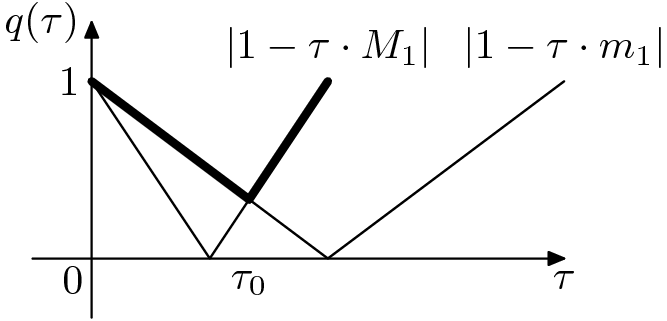
\includegraphics[width=.5\linewidth]{mal-1.png}
\end{figure}

% u:=1cm;
% label.llft(btex $0$ etex, (0,0));
% label.lft(btex $1$ etex, (0,3u/2));
% drawarrow (-u/2,0)--(4u,0);
% drawarrow (0,-u/2)--(0,2u);
% label.lft(btex $q(\tau)$ etex, (0,2u));
% label.bot(btex $\tau$ etex, (4u,0));
% draw (0,3u/2)--(u,0)--(2u,3u/2);
% draw (0,3u/2)--(2u,0)--(4u,3u/2);
% label.top(btex $|1-\tau \cdot M_1|$ etex, (2u,3u/2));
% label.top(btex $|1-\tau \cdot m_1|$ etex, (4u,3u/2));
% draw (4/3u,u/2)--(2u,3u/2) withpen pencircle scaled 2bp;
% draw (0,3u/2)--(4/3u,u/2) withpen pencircle scaled 2bp;
% label.bot(btex $\tau_0$ etex, (4/3u,0));

З графіка видно, що точка мінімуму визначається умовою $|1 - \tau \cdot M_1| = |1 - \tau \cdot m_1|$. \\

Тому
\[ 1 - \tau_0 \cdot m_1 = \tau_0 \cdot M_1 - 1 \Rightarrow \tau_0 = \dfrac{2}{M_1+m_1} < \dfrac{2}{|f'(x)|}.\]

При цьому значенні $\tau$ маємо \[q(\tau_0) = q_0 =\dfrac{M_1-m_1}{M_1+m_1}.\]

Тоді для похибки вірна оцінка \[|x_n-\overline{x}|\le \dfrac{q_0^n\cdot (b-a)}{1-q_0}<\epsilon.\]

Кількість ітерацій \[n = n(\epsilon) \ge \left\lfloor \dfrac{\ln \left(\dfrac{\epsilon\cdot(1-q_0)}{b-a}\right)}{\ln q_0} \right\rfloor + 1.\]	

\begin{problem} 
	Дати геометричну інтерпретацію методу простої ітерації для випадків:
	\[ 0 < \phi'(x) < 1; \quad -1 < \phi'(x) < 0; \quad \phi'(x) < -1; \quad \phi'(x) > 1,\]
\end{problem}

\begin{problem} 
	Знайти оптимальне $\tau = \tau_0$ для методу релаксації при $f'(x) > 0$.
\end{problem}

\subsection{Метод Ньютона (метод дотичних)}

Припустимо, що рівняння $f (x) = 0$ має простий дійсний корінь $\overline{x}$, тобто $f (\overline{x}) = 0$, $f'(\overline{x}) \ne 0$. Нехай виконуються умови: $f (x)\in C^{(1)}([a,b])$, $f (a)\cdot f (b) < 0$. Тоді 
\[0 = f (\overline{x}) = f (x_k + \overline{x} - x_k ) = f (x_k ) + f'(\xi_k ) \cdot (\overline{x} - x_k ),\] 
де $\xi_k=x_k+\theta_k \cdot (\overline{x}-x_k)$, $0 < \theta_k < 1$, $\xi_k \approx x_k$. Тому наступне наближення виберемо з рівняння 
\[ f(x_k) + f'(x_k) \cdot (x_{k+1}-x_k) = 0.\]

Звідси маємо ітераційний процес
\[ x_{k+1} = x_k - \dfrac{f(x_k)}{f'(x_k)}, \quad k = 0,1,2,\ldots, \quad x_0\text{ -- задане}. \]

Метод Ньютона ще називають методом лінеаризації або методом дотичних.

\begin{problem} 
	Дати геометричну інтерпретацію методу Ньютона.
\end{problem}

Метод Ньютона можна інтерпретувати як метод простої ітерації з \[ \phi(x) = x - \dfrac{f(x)}{f'(x)}, \quad \text{тобто} \quad \tau(x) = - \dfrac{1}{f'(x)}. \]

Тому 
\[ \phi'(x) = 1 - \dfrac{f'(x)\cdot f'(x)-f(x)\cdot f''(x)}{(f'(x))^2} = \dfrac{f(x)\cdot f''(x)}{(f'(x))^2}.\]
Якщо $\overline{x}$ -- корінь $f(x)$, то $\phi'(x) = 0$. Тому знайдеться окіл кореня, де \[ |\phi'(x)| = \left|\dfrac{f(x)\cdot f''(x)}{(f'(x))^2}\right|<1.\]

Це означає, що збіжність методу Ньютона залежить від вибору $x_0$. \\

Недолік методу Ньютона: необхідність обчислювати на кожній ітерації не тільки значення функції, а й похідної. \\

Модифікований метод Ньютона позбавлений цього недоліку і має вигляд:
\[ x_{k+1} = x_k - \dfrac{f(x_k)}{f'(x_0)}, \quad k=0,1,2,\ldots. \]

Цей метод має лише лінійну збіжність: $|x_{k+1} - \overline{x}| = O(|x_k-\overline{x}|)$.
\begin{problem} 
	Дати геометричну інтерпретацію модифікованого методу Ньютона.
\end{problem}

В методі Ньютона, для якого $f'(x_k)$ замінюється на $\frac{f(x_k)-f(x_{k-1})}{x_k-x_{k-1}}$ дає метод січних: \[ x_{k+1} = x_k - \dfrac{x_k-x_{k-1}}{f(x_k)-f(x_{k-1})}\cdot f(x_k), \quad k = 1,2,\ldots, \quad x_0,x_1\text{ -- задані}.\]

\begin{problem} 
	Дати геометричну інтерпретацію методу січних.
\end{problem}

\subsection{Збіжність методу Ньютона}

\begin{theorem}
	Нехай $f(x)\in C^{(2)}([a,b])$, $\overline{x}$ -- простий дійсний корінь рівняння
	\begin{equation}
		\label{eq:2.10}
		f (x) = 0
	\end{equation}
	і $f'(x) \ne 0$ при $x\in U_r= \{x: |x -\overline{x}| < r\}$. Якщо
	\begin{equation}
		\label{eq:2.11}
		\dfrac{M_2\cdot|x_0-\overline{x}|}{2m_1} = q < 1
	\end{equation}
	де $m_1 = \Min_{x\in U_r} |f'(x)|$, $M_2 = \Max_{x\in U_r} |f''(x)|$, то для $x_0 \in U_r$ метод Ньютона 
	\begin{equation}
		\label{eq:2.12}
		x_{k+1} = x_k - \dfrac{f(x_k)}{f'(x_k)}
	\end{equation}
	збігається і має місце оцінка
	\begin{equation}
		\label{eq:2.13}
		|x_n - \overline{x}| \le q^{2^n-1} \cdot |x_0 - \overline{x}|.
	\end{equation}
\end{theorem}

\begin{proof}
	З (\ref{eq:2.12}) маємо 
	\begin{equation}
		\label{eq:2.14}
		x_{k+1} - \overline{x} = x_k - \dfrac{f(x_k)}{f'(x_k)} - \overline{x} = \dfrac{(x_k-\overline{x}) \cdot f'(x_k)-f(x_k)}{f'(x_k)} = \dfrac{F(x_k)}{f'(x_k)},
	\end{equation}
	де $F(x) = (x - \overline{x}) \cdot f'(x) - f (x)$, така, що
	\begin{enumerate}
		\item $F(x) = 0$;
		\item $F'(x) = (x - \overline{x}) \cdot f''(x)$;
	\end{enumerate}
	Тоді \[ F(x_k) = F(\overline{x}) + \Int_{\overline{x}}^{x_k}  F'(t) \diff t = \Int_{\overline{x}}^{x_k}  ((t - \overline{x}) \cdot f''(t)) \diff t . \]

	Так як $(t - x)$ не міняє знак на відрізку інтегрування, то скористаємося теоремою про середнє значення:
	\begin{equation}
		\label{eq:2.15}
		F(x_k) = f''(\xi_k) \Int_{\overline{x}}^{x_k}  (t - \overline{x}) \diff t = \dfrac{(x_k-\overline{x})^2}{2} f''(\xi_k),
	\end{equation}
	де $\xi_k = \overline{x} + \theta_k \cdot (x_k - \overline{x})$, $0 <\theta_k < 1$. З (\ref{eq:2.14}), (\ref{eq:2.15}) маємо
	\begin{equation}
		\label{eq:2.16}
		x_{k+1} - \overline{x} = \dfrac{(x_k-\overline{x})^2}{2f'(x_k)} f''(\xi_k).
	\end{equation}
	Доведемо оцінку (\ref{eq:2.12}) за індукцією. Так як $x_0 \in U_r$, то \[|\xi_0 - \overline{x}| = |\theta_0 \cdot (x_0 - \overline{x})| < |\theta_0| \cdot |x_0 - \overline{x}| < r \Rightarrow \xi_0 \in U_r.\]

	Тоді $f''(\xi_0) \le M_2$, тому
	\begin{multline*} 
		|x_1 - \overline{x}| \le \dfrac{(x_0-\overline{x})^2 \cdot M_2}{2m_1} = \dfrac{M_2\cdot|x_0-\overline{x}|}{2m_1}|x_0-\overline{x}| = \\
		= q\cdot |x_0-\overline{x}|=q\cdot |x_0-\overline{x}|<r \Rightarrow x_1\in U_r.
	\end{multline*}

	Ми довели твердження (\ref{eq:2.13}) при $n = 1$. Нехай воно справджується при $n = k$:
	\[ |x_k - \overline{x}| \le q^{2^k-1}\cdot |x_0 - \overline{x}| < r, \quad |\xi_k - \overline{x}| = |\theta_k \cdot (x_k - \overline{x})| < r. \]

	Тоді $x_k, \xi_k \in U_r$. \\

	Доведемо (\ref{eq:2.13}) для $n = k +1$. З (\ref{eq:2.16}) маємо 
	\begin{multline*}
		|x_{k+1}-\overline{x}| \le \dfrac{|x_k - \overline{x}|^2\cdot M_2}{2m_1} \le \left(q^{2^k-1}\right)^2 \dfrac{|x_0-\overline{x}|^2\cdot M_2}{2m_1} = \\
		= q^{2^{k+1}-2} \dfrac{|x_0-\overline{x}|\cdot M_2}{2m_1}|x_0-\overline{x}| = q^{2^{k+1}-1} \cdot |x_0-\overline{x}|.
	\end{multline*}

	Таким чином (\ref{eq:2.13}) справджується для $n = k +1$. Значить (\ref{eq:2.13}) виконується і для довільного $n$. Таким чином $x_n \xrightarrow[n\to\infty]{} \overline{x}$.
\end{proof}

З (\ref{eq:2.13}) маємо оцінку кількості ітерацій для досягнення точності $\epsilon$:
\[ n \ge \left\lfloor\log_2\left(1+\dfrac{\ln \left(\dfrac{\epsilon}{b-a}\right)}{\ln q}\right) \right\rfloor + 1 .\]

Кажуть, що ітераційний метод має \textit{степінь збіжності} $m$, якщо \[ |x_{k+1}-\overline{x}|=O(|x_k-\overline{x}|^m).\]

Для методу Ньютона 
\[|x_{k+1}-\overline{x}| = \dfrac{|x_k-\overline{x}|^2\cdot|f''(\xi_k)|}{2|f'(x_k)|}| \Rightarrow |x_{k+1}-\overline{x}|=O(|x_k-\overline{x}|^2).\]

Значить степінь збіжності методу Ньютона $m=2$. Для методу простої ітерації і ділення навпіл $m=1$.

\begin{theorem}
	Нехай $f(x)\in C^{(2)}([a,b])$ та $\overline{x}$ -- простий корінь рівняння $f (x) = 0$ а також $\forall x\in[a,b]$: $f'(x) \ne 0$. Якщо $f'(x) \cdot f''(x) > 0$ ($f'(x) \cdot f''(x) < 0$) то для методу Ньютона при $x_0 = b$ послідовність наближень $\{x_k \}$ монотонно спадає (монотонно зростає при $x_0 = a$).
\end{theorem}

\begin{problem}
	Довести теорему при 
	\begin{enumerate}
		\item $f'(x) \cdot f''(x) > 0$;
		\item $f'(x) f''(x) < 0$.
	\end{enumerate}
\end{problem}

\begin{problem}
	Знайти степінь збіжності методу січних.
\end{problem}


Якщо $f(a) \cdot f''(a) > 0$ та $f''(x)$ не міняє знак, то потрібно вибирати $x_0 = a$; при цьому $\{x_k \}\uparrow \overline{x}$. \\

Якщо $f(b) \cdot f''(b) > 0$, то $x_0 = b$; маємо $\{x_k \}\downarrow \overline{x}$. Пояснення на рисунку:

% u := 1cm;
% drawarrow (-u/2, 0)--(4u, 0);
% drawarrow (0, -u/2)--(0, 2u);
% draw (u/2,0)--(u/2,u/8);
% draw (7u/2,0)--(7u/2,u/8);
% label.bot(btex $a$ etex, (u/2, 0));
% label.top(btex $b$ etex, (7u/2, u/8));
% draw (u/2,3u/2){dir -75}..(2u,-u/2){dir 0}..(7u/2,-u/4);
% label.top(btex $x_0 = a$ etex, (2u,u));

% u := 1cm;
% drawarrow (-u/2, 0)--(4u, 0);
% drawarrow (0, -u/2)--(0, 2u);
% draw (u/2,0)--(u/2,u/8);
% draw (7u/2,0)--(7u/2,u/8);
% label.top(btex $a$ etex, (u/2, u/8));
% label.bot(btex $b$ etex, (7u/2, 0));
% draw (u/2,-3u/7){dir 75}..(2u,u)..(7u/2,3u/2);
% label.top(btex $x_0 = a$ etex, (2u,3u/2));

\begin{figure}[H]
	\centering
	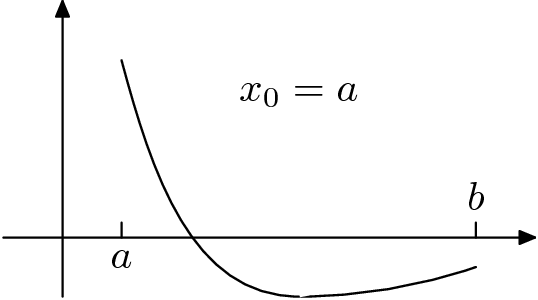
\includegraphics[width=.45\linewidth]{mal-2.png}
	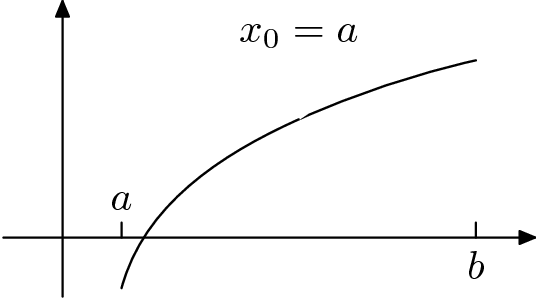
\includegraphics[width=.45\linewidth]{mal-3.png}
\end{figure}

\begin{remark}
	Якщо $\overline{x}$ -- $p$-кратний корінь тобто $f^{(m)} (x) = 0$, $m = \overline{0,p-1}$, $f^{ (p)} (x) \ne 0$, то в методі Ньютона необхідна наступна модифікація \[x_{k+1} = x_k - p\dfrac{f(x_k)}{f'(x_k)} \quad \text{і} \quad q = \dfrac{M_{p+1}\cdot|x_0-\overline{x}|}{m_p \cdot (p+1)}<1.\]
\end{remark}

\begin{remark}
Метод Ньютона можна застосовувати і для обчислення комплексного кореня, тоді ітераційний процес має вигляд \[z_{k+1} = z_k - \dfrac{f(z_k)}{f'(z_k)}, \quad k = 0,1,\ldots.\] В теоремі про збіжність $q = \frac{|z_0-\overline{z}|\cdot M_2}{2m_1}$, де $m_1 = \Min_{z\in U_r} |f'(z)|$, $M_2 = \Max_{z\in U_r} |f''(z)|$. Тут $|z|$ -- модуль комплексного числа $z$.
\end{remark}

Переваги методу Ньютона: 
\begin{enumerate}
\item висока швидкість збіжності;
\item узагальнюється на системи рівнянь; 
\item узагальнюється на комплексні корені.
\end{enumerate}
Недоліки методу Ньютона: 
\begin{enumerate}
	\item на кожній ітерації обчислюється не тільки $f (x_k )$ , а і похідна $f'(x_k)$;
	\item  збіжність залежить від початкового наближення $x_0$, так як від нього залежить умова збіжності $q = \frac{M_2\cdot |x_0-\overline{x}|}{2m_1} < 1$;
	\item потрібно, щоб $f (x)\in C^{(2)}([a,b])$.
\end{enumerate}
% \subsubsection{Характеристики розсіювання значень}
Нехай маємо вибірку об'єму $n$ спостережень $x_1$, $x_2$, $\ldots$, $x_n$ над випадковою величиною $\xi$.
\begin{enumerate}
	\item \textit{Дисперсія} $D\xi = M(\xi - M\xi)^2$. Вибіркове значення \[ S^2(n) = \dfrac{1}{n-1} \sum_{i=1}^n (x_i - \bar{x}(n))^2 = \dfrac{1}{n-1} \left(\sum_{i=1}^n x_i^2 - n\bar{x}^2(n) \right). \]
	\item \textit{Стандартне (середньоквадратичне) відхилення} $\sqrt{D\xi}$. Вибіркове значення $S(n)$.
	\item \textit{Коефіцієнт варіацій} $V_\xi = \frac{\sqrt{D\xi}}{M\xi} 100\%$, $M\xi\ne0$. Вибіркове значення $\widehat{V}_\xi(n)=\frac{S(n)}{\bar x(n)} 100\%$.
	\item \textit{Стохастичне розсіювання} (імовірнісне відхилення) -- це половина інтерквартильної широти: $\frac{U_{0.75} - U_{0.25}}{2}$. Вибіркове значення $\frac{\widehat{U}_{0.75} - \widehat{U}_{0.25}}{2}$.
	\item \textit{Розмах (широта) вибірки}: $x_{\max}-x_{\min}$, де $x_{\max}, x_{\min}$ -- найбільше та найменше значення у вибірці.
	\item \textit{Інтервал концентрації} $(M\xi - 3\sqrt{D\xi}, M\xi + 3 \sqrt{D\xi})$. Вибіркове значення $(\bar x(n) - 3S(n), M\bar x(n) + 3 S(n))$.
\end{enumerate}
\subsubsection{Характеристики скошеності та гостроверхості розподілу}
Нехай є розподіл випадкової величини $\xi$ і отримані спостереження $x_1$, $x_2$, $\ldots$, $x_n$ над нею.
\begin{enumerate}
	\item \textit{Коефіцієнт асиметрії} -- характеристика скошеності розподілу (базується на третьому центральному моменті): \[ \beta_1 = \dfrac{M(\xi - M\xi)^3}{(M(\xi - M\xi)^2)^{3/2}}, \quad D\xi > 0. \] Вибіркове значення \[ \widehat{\beta}_1 = \dfrac{\dfrac{1}{n}\Sum_{i=1}^n(x_k - \bar{x}(n))^3}{S^3(n)}. \] Дисперсія спостережуваної величини $D\xi > 0$. \\ % figure 6

	Якщо розподіл симетричний (наприклад нормальний) то $\beta_1 =0$. Якщо $\beta_1 > 0$, то розподіл скошений вліво, якщо $\beta_1 < 0$, то вправо.
	\item \textit{Коефіцієнт ексцесу} -- характеристика гостроверхості розподілу (базується на четвертому центральному моменті): \[ \beta_2 = \dfrac{M(\xi-M\xi)^4}{(M(\xi-M\xi)^2)^2} - 3, \quad D\xi > 0. \] Вибіркове значення \[ \widehat{\beta}_2 = \dfrac{\dfrac{1}{n}\Sum_{i=1}^n(x_k - \bar{x}(n))^4}{S^4(n)} - 3. \]
	Для нормального розподілу коефіцієнт ексцесу дорівнює нулю. Якщо $\beta_2 > 0$, то розподіл більш гостроверхий ніж нормальний, якщо $\beta_2 < 0$ то відповідно менш гостроверхий.
\end{enumerate}
\subsection{Характеристики векторних величин}
Аналіз $q$-вимірних векторних величин, отримано $n$ спостережень над вектором $\vec\xi: x_1, x_2, \ldots, x_n$, $x_i \in \RR^q$, $i = \overline{1,n}$.
\subsubsection{Характеристики положення центру значень}
\begin{enumerate}
	\item \textit{Математичне сподівання} (теоретичне середнє) $M\xi$. Вибіркове значення \[\bar{x}(n) = \dfrac{1}{n} \Sum_{i=1}^n \vec{x}_i.\]
	\item \textit{Мода} $x_{\text{mod}}$. У неперервному випадку -- це точка максимуму функції щільності $\xi$. Для дискретного випадку -- це значення, яке набуває $\xi$ з найбільшою ймовірністю.
\end{enumerate}
\subsubsection{Характеристики розсіювання значень}
\begin{enumerate} 
	\item \textit{Коваріаційна матриця} $\sum = M(\xi - M\xi)(\xi - M\xi)^T$. Вибіркове значення \[\widehat{\sum}(n) = \dfrac{1}{n-1} \Sum_{k=1}^n (x_k - \bar x(n))(x_k - \bar x(n))^T.\]
	\item \textit{Узагальнена дисперсія} -- визначник коваріаційної матриці: $\det \sum$. Вибіркове значення $\det\left(\widehat{\sum}\right)$.
	\item \textit{Слід коваріаційної матриці} $\trace\sum$. Вибіркове значення $\trace\left(\widehat{\sum}(n)\right)$.
\end{enumerate}
\subsection{Перевірка стохастичності вибірки}
Перевіряємо, чи справді вибірка є випадковою, а не знаходиться під впливом деякого систематичного зміщення. Для цього запропоновано критерії:
\begin{itemize}
	\item Критерій серій на базі медіани
	\item Критерій зростаючих та спадаючих серій
	\item Критерій квадратів послідовних різниць (критерій Аббе)
\end{itemize}
Нехай $x_1$, $x_2$, $\ldots$, $x_n$ -- вибірка спостережень, яка досліджується. \\

Будемо перевіряти гіпотезу $H_0$: ця вибірка є стохастичною з рівнем значимості $\alpha (0 < \alpha < 1$) (рівень значимості -- ймовірність допустити помилку першого роду).
\begin{enumerate}
	\item \textit{Критерій серій на базі медіани}. Альтернативна гіпотеза $H_1$: наявність у вибірці систематичного монотонного зміщення середнього. \\

	Спочатку визначається вибіркове значення медіани $\widehat{x}_{\text{med}}$. Потім під кожним членом вибірки ставимо відповідно \[ \begin{cases} +, & x_i > \widehat{x}_{\text{med}} \\
 \text{нічого}, & x_i = \widehat{x}_{\text{med}} \\
 -, & x_i < \widehat{x}_{\text{med}} \end{cases}. \]
	Отримаємо послідовність символів. \textit{Серія} -- послідовність підряд розташованих однакових символів $+$ чи $-$. \textit{Довжина серії} -- це кількість членів у ній. \\

	Для отриманої послідовності обчислюємо дві статистики: загальну кількість серій в послідовності $v(n)$, довжину найдовшої серії $\tau(n)$. Запишемо область прийняття нашої гіпотези: \[ \left\{ \begin{matrix} v(n) > v_\beta(n) \\
 \tau(n) < \tau_{1-\beta}(n) \end{matrix} \right. \] 
	де $v_\beta(n)$, $\tau_\beta(n)$ -- квантилі рівня $\beta$ статистик $v(n)$, $\tau(n)$ відповідно. При фіксованому значенні $\beta$ рівень значимості $\alpha$ лежить у межах $\beta < \alpha < 2\beta - \beta^2$. Якщо порушується хоч одна з нерівностей, то гіпотеза відхиляється.
	\item \textit{Критерій зростаючих та спадаючих серій}. Альтернативна гіпотеза $H_1$: наявність у вибірці систематичного періодичного зміщення середнього. Спочатку у вибірці замінюємо підряд розташовані однакові виміри одним їх представником. В результаті отримаємо послідовність $x_1'$, $x_2'$, $\ldots$, $x_k'$. Під кожним членом послідовності ставимо відповідно \[ \begin{cases} +, & x_i' < x_{i+1}' \\
 -, & x_i' > x_{i+1}' \end{cases}. \]
	Далі для таким чином отриманої послідовності $+$ та $-$, як і в попередньому випадку, обчислюємо дві статистики: загальну кількість серій в послідовності $v(n)$, довжину найдовшої серії $\tau(n)$. Запишемо область прийняття нашої гіпотези: \[ \left\{ \begin{matrix} v(n) > v_\beta(n) \\
 \tau(n) < \tau_{1-\beta}(n) \end{matrix} \right. \] де $v_\beta(n)$, $\tau_\beta(n)$ -- квантилі рівня $\beta$ статистик $v(n)$, $\tau(n)$ відповідно. При фіксованому значенні $\beta$ рівень значимості $\alpha$ лежить у межах $\beta < \alpha < 2\beta - \beta^2$. Якщо порушується хоч одна з нерівностей, то гіпотеза відхиляється.
	\item \textit{Критерій квадратів послідовних різниць (критерій Аббе)}. Він є найбільш потужним на класі усіх нормальних вибірок. Альтернативна гіпотеза $H_1$: наявність у вибірці систематичного зміщення середнього. \\

	На основі вибірки підраховуємо наступну статистику: \[ \gamma(n) = \dfrac{\dfrac{1}{2(n-1)} \Sum_{i=1}^{n-1} (x_{i+1}-x_i)^2}{\dfrac{1}{n-1}\left(\Sum_{i=1}^n x_i^2 - n \bar{x}^2(n)\right)}. \]
	Область прийняття гіпотези для цього критерію має вигляд $\gamma(n) > \gamma_\alpha(n)$, де $\gamma_\alpha(n)$ -- квантиль рівня $\alpha$ статистики $\gamma(n)$, що при $n \le 60 $визначається з таблиць, а протилежному випадку потрібно скористатися формулою \[\gamma_\alpha(n) = 1 + \dfrac{u_\alpha}{\sqrt{n + 0.5(1 + u_\alpha^2)}}, \] де $u_\alpha$ -- квантиль рівня $\alpha$ нормального розподілу з параметрами 0 та 1.
\end{enumerate}
% \section{Ітераційні методи для систем}

\subsection{Ітераційні методи розв'язання СЛАР}

Систему
\begin{equation}
	\label{eq:4.1}
	A \vec x = \vec b
\end{equation}
зводимо до вигляду
\begin{equation}
	\label{eq:4.2}
	\vec x = B \vec x + \vec f.
\end{equation}
Будь яка система
\begin{equation}
	\label{eq:4.3}
	\vec x = \vec x - C \cdot (A \vec x - \vec b)
\end{equation}
має вигляд (\ref{eq:4.2}) і при $\det C \ne 0$ еквівалентна системі (\ref{eq:4.1}). Наприклад, для $C = \tau \cdot E$:
\begin{equation}
	\label{eq:4.4}
	\vec x = \vec x - \tau \cdot (A \vec x - \vec b).
\end{equation}


\subsubsection{Метод простої ітерації}

Цей метод застосовується до рівняння (\ref{eq:4.2})
\begin{equation}
	\label{eq:4.5}
	\vec x^{(k+1)} = B \vec x^{(k)} + \vec f,
\end{equation}
де $\vec x^{(0)}$ -- початкове наближення, задано.\\

Ітераційний процес збігається, тобто $\left\| \vec x^{(k)} - \vec x\right\| \xrightarrow[k\to\infty]{} 0$, якщо
\begin{equation}
	\label{eq:4.6}
	\|B\| \le q < 1
\end{equation}
При цьому має місце оцінка
\begin{equation}
	\label{eq:4.7}
	\left\|\vec x^{(n)} - \vec x\right\| \le \dfrac{q^n}{1-q}\cdot\left\|\vec x^{(1)} - \vec x^{(0)}\right\|.
\end{equation}

\subsubsection{Метод Якобі}

Припустимо $\forall i$: $a_{i,i} \ne 0$. Зведемо систему (\ref{eq:4.1}) до вигляду
\[ x_i = -\Sum_{j=1}^{i-1} \dfrac{a_{i,j}}{a_{i,i}} \cdot x_j - \Sum_{j=i+1}^n \dfrac{a_{i,j}}{a_{i,i}} \cdot x_j + \dfrac{b_i}{a_{i,i}}, \quad i=\overline{1,n}. \]

Ітераційний процес запишемо у вигляді
\begin{equation}
	\label{eq:4.8}
	x_i^{(k+1)} = -\Sum_{j=1}^{i-1} \dfrac{a_{i,j}}{a_{i,i}} \cdot x_j^{(k)} - \Sum_{j=i+1}^n \dfrac{a_{i,j}}{a_{i,i}} \cdot x_j^{(k)} + \dfrac{b_i}{a_{i,i}}, \quad k = 0,1,\ldots, \quad i=\overline{1,n}.
\end{equation}

Ітераційний процес збігається до розв’язку, якщо виконується умова
\[ \forall i: \Sum_{\substack{j = 1 \\ i \ne j}}^n |a_{i,j}| \le |a_{i,i}|. \]

Це умова діагональної переваги матриці $A$. Якщо ж
\begin{equation}
	\label{eq:4.9}
	\forall i: \Sum_{\substack{j = 1 \\ i \ne j}}^n |a_{i,j}| \le q\cdot|a_{i,i}|, \quad 0 \le q < 1.
\end{equation}
то має місце оцінка точності:
\[ \|\vec x^{(n)} - \vec x\| \le \dfrac{q^n}{1-q}\cdot\|\vec x^{(0)}-\vec x\|. \]

\subsubsection{Метод Зейделя}
В компонентному вигляді ітераційний метод Зейделя записується так:
\begin{equation}
	\label{eq:4.10}
	x_i^{(k+1)} = -\Sum_{j=1}^{i-1} \dfrac{a_{i,j}}{a_{i,i}} \cdot x_j^{(k+1)} - \Sum_{j=i+1}^n \dfrac{a_{i,j}}{a_{i,i}} \cdot x_j^{(k)} + \dfrac{b_i}{a_{i,i}}, \quad k = 0,1,\ldots, \quad i=\overline{1,n}.
\end{equation}

На відміну від методу Якобі на $k$-му-кроці попередні компоненти розв'язку беруться з $k+1$-ої ітерації. \\

Достатня умова збіжності методу Зейделя -- $A^T = A > 0$.

\subsubsection{Матрична інтерпретація методів Якобі і Зейделя}

Подамо матрицю $A$ у вигляді \[ A = A_1 + D + A_2, \]
де $A_1$ -- нижній трикутник матриці $A$, $A_2$ -- верхній трикутник матриці $A$, $D$ -- її
діагональ. Тоді систему (\ref{eq:4.1}) запишемо у вигляді \[ D \vec x = A_1 \vec x + A_2 \vec x + \vec b,\]
або
\[ \vec x = D^{-1} A_1 \vec x + D^{-1} A_2 \vec x + D^{-1} \vec b,\]
 
Матричний запис методу Якобі:
\[ \vec x^{(k+1)} = D^{-1} A_1 \vec x^{(k)} + D^{-1} A_2 \vec x^{(k)} + D^{-1} \vec b,\]
методу Зейделя:
\[ \vec x^{(k+1)} = D^{-1} A_1 \vec x^{(k+1)} + D^{-1} A_2 \vec x^{(k)} + D^{-1} \vec b,\]

Необхідна і достатня умова збіжності методу Якобі: всі корені рівняння \[\det(D + \lambda(A_1 + A_2 )) = 0\] по модулю більше 1. \\

Необхідна і достатня умова збіжності методу Зейделя: всі корені рівняння \[\det(A_1 + D + \lambda A_2) = 0\] по модулю більше 1.

\subsubsection{Однокрокові (двошарові) ітераційні методи}

Канонічною формою однокрокового ітераційного методу розв'язку СЛАР є його запис у вигляді
\begin{equation}
	\label{eq:4.11}
	B_k \dfrac{\vec x^{(k+1)} - \vec x^{(k)}}{\tau_{k+1}} + A \vec x^{(k)} = \vec b,
\end{equation}

Тут $\{B_k\}$ -- послідовність матриць (пере-обумовлюючі матриці), що задають ітераційний метод на кожному кроці; $\{\tau_{k+1}\}$ -- ітераційні параметри. \\

Якщо $B_k = E$, то ітераційний процес називається \textit{явним}
\[ \vec x^{(k+1)} = \vec x^{(k)} - \tau_{k+1} \left(A \vec x^{(k)} + \vec b\right). \]
Якщо $B_k \ne E$, то ітераційний процес називається \textit{неявним}
\[ B_k \vec x^{(k+1)} = F^k. \]

У цьому випадку на кожній ітерації необхідно розв'язувати СЛАР. \\

Якщо $\tau_{k+1} \equiv \tau$, $B_k \equiv B$, то ітераційний процес називається \textit{стаціонарним}; інакше -- \textit{нестаціонарним}. \\

Методам, що розглянуті вище відповідають:
\begin{itemize}
	\item методу простої ітерації: $B_k = E$, $\tau_{k+1} = \tau$;
	\item методу Якобі: $B_k = D$, $\tau_{k+1} = 1$.;
	\item методу Зейделя: $B_k = D + A_1$, $\tau_{k+1} = 1$.
\end{itemize}

\subsubsection{Збіжності стаціонарних ітераційних процесів у випадку симетричних матриць}

Розглянемо випадок симетричних матриць $A^T=A$ і стаціонарний ітераційний процес $B_k \equiv E$, $\tau_{k+1} \equiv \tau$. \\

Нехай для $A$ справедливі нерівності
\begin{equation}
	\label{eq:4.12}
	\gamma_1 E \le A \le \gamma_2 E, \quad \gamma_1, \gamma_2 > 0.
\end{equation}

Тоді при виборі $\tau = \tau_0 = \frac{2}{\gamma_1 + \gamma_2}$ ітераційний процес збігається. Найбільш точним значенням $\gamma_1$, $\gamma_2$ при яких виконуються обмеження (\ref{eq:4.12}) є $\gamma_1 = \min \lambda_i(A)$, $\gamma_2 = \max \lambda_i(A)$. Тоді 
\[q = q_0 = \dfrac{\gamma_2 - \gamma_1}{\gamma_2 + \gamma_1} = \dfrac{1-\xi}{1+\xi}, \quad \xi = \dfrac{\gamma_1}{\gamma_2}.\]
(Зауважимо, що аналогічно обчислюється $q$ і для методу релаксації розв'язання нелінійних рівнянь, де $\gamma_1 = m = \min |f'(x)|$, $\gamma_2 = M_1 = \max|f'(x)|$) і справедлива оцінка\[ \|\vec x^{(n)} - \vec x\| \le \dfrac{q^n}{1-q} \cdot \|\vec x^{(0)} - \vec x\|. \]

Явний метод з багатьма параметрами $\{\tau_k\}$:
\[ B \equiv E, \quad \{\tau_k\}: \Min_\tau q(\tau), \quad n=n(\epsilon)\to\min,\]
які обчислюються за допомогою нулів багаточлена Чебишова, називаються ітераційним методом з чебишевським набором параметрів.

\subsubsection{Метод верхньої релаксації}

Узагальненням методу Зейделя є метод верхньої релаксації: \[ (D + \omega A_1) \cdot\dfrac{\vec x^{(k+1)} + \vec x^{(k)}}{\omega} + A \vec x^{(k)} = \vec b,\]
де $D$ -- діагональна матриця з елементами $a_{i,i}$ по діагоналі. $\omega > 0$ -- заданий числовий параметр. \\

Тепер $B = D + \omega A_1$, $\tau = \omega$. Якщо $A^T = A > 0$, то метод верхньої релаксації збігається при умові $0 < \omega < 2$. Параметр підбирається експериментально з умови мінімальної кількості ітерацій. 

\subsubsection{Методи варіаційного типу}

До цих методів відносяться: метод мінімальних нев’язок, метод мінімальних поправок, метод найшвидшого спуску, метод спряжених градієнтів. Вони дозволяють обчислювати наближення без використання апріорної інформації про $\gamma_1$, $\gamma_2$ в (\ref{eq:4.12}). \\

Нехай $B = E$. Для методу мінімальних нев’язок параметри $\tau_{k+1}$ обчислюються з умови 
\[ \left\|\vec r^{(k+1)}\right\|^2 = \left\|\vec r^{(k)}\right\|^2 - 2\tau_{k+1}\cdot\left(\vec r^{(k)}, A\vec r^{(k)}\right) + \tau_{k+1}^2 \cdot\left\|A\vec r^{(k)}\right|^2 \to \min. \]

Тому \[ \tau_{k+1} = \dfrac{\left(A\vec r^{(k)}, \vec r^{(k)}\right) }{\left\|\vec r^{(k)}\right\|^2},\] 
де $\vec r^{(k)} = A \vec x^{(k)} - \vec b$ -- нев'язка. \\

Умова для завершення ітераційного процесу: \[ \left\|\vec r^{(n)}\right\| < \epsilon.\]

Швидкість збіжності цього методу співпадає із швидкістю методу простої ітерації з одним оптимальним параметром $\tau_0 = \frac{2}{\gamma_1+\gamma_2}$. \\

Аналогічно будуються методи з $B \ne E$. Матриця $B$ називається переобумовлювачем і дозволяє підвищити швидкість збіжності ітераційного процесу. Його вибирають з умов 
\begin{enumerate}
	\item легко розв’язувати СЛАР $B \vec x^{(k)} = F_k$ (діагональний, трикутній, добуток трикутніх та інше); 
	\item зменшення числа обумовленості матриці $B^{-1}A$ у порівнянні з $A$.
\end{enumerate}

\subsection{Методи розв’язання нелінійних систем}

Розглянемо систему рівнянь
\[ \left\{ \begin{aligned} & f_1(x_1, \ldots, x_n) = 0, \\ & \ldots \\ & f_n(x_1,\ldots,x_n) = 0. \end{aligned} \right. \]

Перепишемо її у векторному вигляді: 
\begin{equation}
	\label{eq:4.13}
	\vec f(\vec x) = 0.
\end{equation}

\subsubsection{Метод простої ітерації}

В цьому методі рівняння (\ref{eq:4.13}) зводиться до еквівалентного вигляду
\begin{equation}
	\label{eq:4.14}
	\vec x = \vec \Phi(\vec x).
\end{equation}

Ітераційний процес представимо у вигляді:
\begin{equation}
	\label{eq:4.15}
	\vec x^{(k+1)} = \vec \Phi\left(\vec x^{(k)}\right).
\end{equation}
початкове наближення $\vec x^{(0)}$ -- задано. \\

Нехай оператор $\vec \Phi$ визначений на множині $H$. За теоремою про стискуючі відображення ітераційний процес (\ref{eq:4.15}) сходиться, якщо виконується умова
\begin{equation}
	\label{eq:4.16}
	\left\| \vec \Phi(\vec x) - \vec \Phi(\vec y) \right\| \le q \cdot \|\vec x - \vec y\|, \quad 0 < q < 1, 
\end{equation}
або
\begin{equation}
	\label{eq:4.17}
	\left\| \vec \Phi'(\vec x)\right\| \le q < 1, 
\end{equation}
де $\vec x\in U_r$, $\vec \Phi'(\vec x) = \left(\frac{\partial \phi_i}{\partial x_j}\right)_{i,j=1}^n$. Для похибки справедлива оцінка
\[ \left\| \vec x^{(m)} - \vec x\right\| \le \dfrac{q^n}{1 - q} \cdot\left\|\vec x^{(0)} - \vec x\right\|.\]

Частинним випадком методу простої ітерації є метод релаксації для рівняння (\ref{eq:4.13}):
\[ \vec x^{(k+1)} = \vec x^{(k)} - \tau \cdot \vec F\left(\vec x^{(k)}\right), \]
де $\tau < \frac{2}{\left\|\vec F'(\vec x)\right\|}$.

\subsubsection{Метод Ньютона}

Розглянемо рівняння
\[ \vec F(\vec x) = 0. \]

Представимо його у вигляді
\begin{equation}
	\label{eq:4.18}
	\vec F\left(\vec x^{(k)}\right) + \vec F'\left(\vec \xi^{(k)}\right)\cdot\left(\vec x - \vec x^{(k)}\right) = 0,
\end{equation}
де $\vec \xi^{(k)} = \vec x^{(k)} + \theta_k \cdot \left(\vec x^{(k)} - \vec x\right)$, $0 < \theta_k < 1$. Тут  $\vec F'(\vec x) = \left(\frac{\partial f_i}{\partial x_j}\right)_{i,j=1}^n$ -- матриця Якобі для $\vec F(\vec x)$. Можемо наближено вважати $\vec \xi^{(k)} \approx \vec x^{(k)}$. Тоді з (\ref{eq:4.18}) матимемо
\begin{equation}
	\label{eq:4.19}
	\vec F\left(\vec x^{(k)}\right) + \vec F'\left(\vec x^{(k)}\right) \cdot\left(\vec x^{(k+1)} - \vec x^{(k)}\right) = 0.
\end{equation}
Ітераційний процес представимо у вигляді:
\begin{equation}
	\label{eq:4.20}
	\vec x^{(k+1)} = \vec x^{(k)} - \vec F'\left(\vec x^{(k)}\right)^{-1} \cdot \vec F\left(\vec x^{(k)}\right). 
\end{equation}

Для реалізації методу Ньютона потрібно, щоб існувала обернена матриця \[\vec F'\left(\vec x^{(k)}\right)^{-1}. \]

Можна не шукати обернену матрицю, а розв’язувати на кожній ітерації СЛАР
\begin{equation}
	\label{eq:4.21}
	\left\{
		\begin{aligned}
			& A_k \vec z^{(k)} = \vec F\left(\vec x^{(k)}\right), \\
			& \vec x^{(k + 1)} = \vec x^{(k)} - \vec z^{(k)},
		\end{aligned}
		\quad k=0,1,2,\ldots
	\right.
\end{equation}
де $\vec x^{(0)}$ -- задано, а матриця $A_k = \vec F'\left(\vec x^{(k)}\right)$. \\

Метод має квадратичну збіжність, якщо добре вибрано початкове наближення. Складність методу (при умові використання методу Гаусса розв'язання СЛАР (\ref{eq:4.21}) на кожній ітерації $Q_n = \frac23 n^3+O(n^2)$, де $n$ -- розмірність системи (\ref{eq:4.13}).

\subsubsection{Модифікований метод Ньютона}

Ітераційний процес має вигляд :
\[ \vec x^{(k+1)} = \vec x^{(k)} - \vec F'\left(\vec x^{(0)}\right)^{-1} \cdot\vec F\left(\vec x^{(k)}\right). \]

Тепер обернена матриця обчислюється тільки на нульовій ітерації. На інших -- обчислення нового наближення зводиться до множення матриці $A_0 = \vec F'\left(\vec x^{(0)}\right)^{-1}$ на вектор $\vec F\left(\vec x^{(k)}\right)$ та додавання до $\vec x^{(k)}$. \\

Запишемо метод у вигляді системи лінійних рівнянь (аналог (\ref{eq:4.21}))
\begin{equation}
	\label{eq:4.22}
	\left\{
		\begin{aligned}
			& A_0 \vec z^{(k)} = \vec F\left(\vec x^{(k)}\right), \\
			& \vec x^{(k + 1)} = \vec x^{(k)} - \vec z^{(k)},
		\end{aligned}
		\quad k=0,1,2,\ldots
	\right.
\end{equation}
Оскільки матиця $A_0$ розкладається на трикутні (або обертається) один раз, то складність цього методу на одній ітерації (окрім нульової) $Q_n = O(n^2)$. Але цей метод має лінійну швидкість збіжності. \\

Можливе циклічне застосування модифікованого методу Ньютона, тобто коли обернену матрицю похідних шукаємо та обертаємо через певне число кроків ітераційного процесу. \\

\begin{problem}
	Побудувати аналог методу січних для систем нелінійних рівнянь.
\end{problem}
% \subsection{Коефіцієнт кореляції}
Розглянемо нормальний випадок. Є дві величини $\xi$ та $\eta$. \[\xi \sim N(m_\xi, \sigma_\xi^2), x_1, \ldots, x_n \qquad \eta \sim N(m_\eta, \sigma_\eta^2), y_1, \ldots, y_n \qquad. \]
\[ r_{\eta\xi} = \dfrac{M(\xi-M\xi)(\eta-M\eta)}{\sqrt{D\xi D\eta}}, \] вибіркове значення:
\[ \widehat{r}_{\eta\xi} = \dfrac{\Sum_{i=1}^n(x_i-\bar{x}(n))(y_i-\bar{y}(n))}{\sqrt{\Sum_{i=1}^n(x_i-\bar{x}(n))^2\Sum_{i=1}^n(y_i-\bar{y}(n))^2}}. \]
Можна довести, що $I_{\eta\xi}=|r_{\eta\xi}$. \\

\textbf{Властивості}:
\begin{enumerate}
	\item $|r_{\eta\xi}| \le 1$.
	\item якщо $r_{\eta\xi} = 0$ то зв'язок між $\eta$ і $\xi$ відсутній.
	\item Якщо $r_{\eta\xi} = \pm 1$ то зв'язок між $\eta$ і $\xi$ лінійний, причому \textit{формула зв'язку}: $\eta = m_\eta + r_{\eta\xi}\sigma_\eta \dfrac{\xi - m_\xi}{\sigma_\xi}$.
	\item Нехай $r_{\eta\xi} > 0$. Якщо $\xi \uparrow$, то і $\eta \uparrow$.
	\item Нехай $r_{\eta\xi} < 0$. Якщо $\xi \uparrow$, то $\eta \downarrow$.
	\item Якщо коефіцієнт кореляції прийняв проміжне значення, то перевіряємо гіпотезу $H_0$: $r_{\eta\xi} = 0$, $0 < \alpha < 1$. Для перевірки $H_0$ будемо розглядати статистику: \[t(n-2)=\dfrac{\sqrt{n-2}r_{\eta\xi}}{\sqrt{1-r_{\eta\xi}^2}}. \]
	Ця статистика має асимптотичний $t$-розподіл Стьюдента з $(n - 2)$ степенями свободи. Тоді логічно вважати, що $H_0$ гіпотеза несправедлива, коли статистика приймає екстремальні значення. $|t(n-2)| < t_{\alpha/2}(n-2)$ -- область прийняття гіпотези $H_0$, де $t_\alpha(n)$ -- $100\alpha\%$ -- точки $t$-розподілу Стьюдента з $v$ степенями свободи.
\end{enumerate}
\subsection{Характеристика парного статистичного зв'язку в загальному випадку}
Нехай спостерігаються $\xi$ і $\eta$, з'ясуємо наявність зв'язку. Розглянемо 2 випадки:
\begin{itemize}
	\item випадок групованих (за $\xi$) даних;
	\item випадок не згрупованих даних.
\end{itemize}
\begin{enumerate}
	\item Спостереження над залежною змінною $\eta$: $y_{11}$, $\ldots$, $y_{1m_1}$, $\ldots$, $y_{s1}$, $\ldots$, $y_{sm_s}$, $s$ інтервалів групування, в $i$-му інтервалі $m_i$ спостережень. \\

	$\bar{y}_i$ --  вибіркове середнє спостережень по групі $i$, $\bar{y}$ -- загальне вибіркове середнє. \\

	$S_y^2$ -- вибіркове значення дисперсії $\eta$, $S_{y(x)}^2$ -- зважене вибіркове значення дисперсії вибіркових середніх $\bar{y}_i$. \\

	Запишемо оцінку для індексу кореляції (кореляційне відношення): \[\widehat{p}_{\eta\xi}=\sqrt{\dfrac{S_{y(x)}^2}{S_y^2}}.\] Властивості такі ж, як і в індексу кореляції. З'ясувалося, що
	\[ F = \dfrac{\widehat{p}_{\eta\xi}^2}{1 - \widehat{p}_{\eta\xi}^2} \cdot \dfrac{n - s}{s - 1} \] має асимптотичний розподіл, який тотожньо рівний $F(s - 1, n - s)$. Припускаємо, що спостереження нормальні. \\

	\textit{Область прийняття гіпотези}: $F < F_\alpha(s - 1, n  -s)$, де $F_\alpha$ -- $100\alpha\%$-точка $F$-розподілу з параметрами $s - 1$, $n - s$.
	\item Функцію регресії $f$ апроксимують на деякому класі параметричних функцій з точністю до вектор-параметру $\theta$. $f (x,\theta),\theta \in\RR^p$. \\

	По спостереженням досліджуваних змінних: $\xi: x_1, \ldots, x_n$, $\eta: y_1, \ldots, y_n$. \\

	Методом найменших квадратів визначаємо $\widehat{\theta}$, далі отримуємо деяку апроксимацію функції регресії $f (x,\theta)$. \\

	Апроксимація індексу кореляції даних у вигляді:
	\[ \widehat{I}_{\eta\xi} = \sqrt{1 - \dfrac{\dfrac{1}{n-p} \Sum_{i=1}^n (y_i - f(x_i, \widehat{\theta}))^2}{\dfrac{1}{n-1}\Sum_{i=1}^n (y_i-\bar{y}(n))^2}}. \]
	\textbf{Приклад $\theta$}: $f(x, \theta) = \Sum_{i=1}^N \theta_i f_i(x)$.
\end{enumerate}
\subsection{Частинний коефіцієнт кореляції}
\textit{Частинним коефіцієнтом кореляції} для змінних $x^{(i)}$, $x^{(j)}$ будемо називати величину: \[r_{ij}^* = - \dfrac{R_{ij}}{\sqrt{R_{ii}R_{jj}}},\] де $R_{ij}$ -- алгебраїчне доповнення для елемента $(i, j)$ у звичайній кореляційній матриці: \[ R = \begin{pmatrix} 1 & r_{01} & \ldots & r_{0q} \\
 r_{10} & 1 & \ldots & r_{1q} \\
 \vdots & \vdots & \ddots & \vdots \\
 r_{q0} & r_{q1} & \ldots & 1 \end{pmatrix}, \] де $r_{ij}$ -- звичайний коефіцієнт кореляції. \\

Властивості частинного співпадають з властивостями звичайного коефіцієнта кореляції. Вибіркове значення коефіцієнта кореляції: \[\widehat{r}_{ij}^* = - \dfrac{\widehat{R}_{ij}}{\sqrt{\widehat{R}_{ii}\widehat{R}_{jj}}},\] \[ \widehat{R} = \begin{pmatrix} 1 & \widehat{r}_{01} & \ldots & \widehat{r}_{0q} \\
 \widehat{r}_{10} & 1 & \ldots & \widehat{r}_{1q} \\
 \vdots & \vdots & \ddots & \vdots \\
 \widehat{r}_{q0} & \widehat{r}_{q1} & \ldots & 1 \end{pmatrix}. \]
При $r_{ij}^* = 0$ зв'язку не існує. \\

При $r_{ih}^* = \pm1$ то зв'язок функціональний. \\

Якщо коефіцієнт прийняв проміжне значення, то перевіряється гіпотеза $H_0$: $r_{ij}^*=0$, $\alpha>0$.  Використовуємо статистику: \[t(n - m - 2) = \dfrac{\sqrt{n - m - 2}\cdot \widehat{r}_{ij}^*}{\sqrt{1 - (\widehat{r}_{ij}^*)^2}},\] де $m$ -- кількість третіх змінних зафіксованих на певному рівні. \\

Вона має $t$-розподіл Стьюдента з $n - m - 2$ степенями свободи. Критична область -- обасть великих і малих значень. \textit{Область прийняття} має вигляд: \[|t(n - m - 2)| < t_{\alpha/2}(n - m - 2),\] де $t_{\alpha/2}(n - m - 2)$ -- $100\alpha/2\%$ точка $t$-розподілу Стьюдента з $n - m - 2$ степенями свободи.
\subsection{Множинний коефіцієнт кореляції}
Розглянемо залежну змінну $\eta$ і незалежну змінну $\vec\xi\in\RR^q$. Для з'ясування зв'язку
використовується \textit{множинний коефіцієнт кореляції}: \[R_{\eta\xi} = \sqrt{D(f\xi)}{D\eta}=\sqrt{1-\dfrac{M(g(\xi))}{D\eta}},\] де умовні матсподівання і дисперсія визначаються так же як і раніше тільки для векторної $\xi$. \\

\textit{Множинний коефіцієнт детермінації}: $R_{\eta\xi}^2$. \\

Властивості множинного коефіцієнта кореляції такі ж, як і звичайного коефіцієнта кореляції. \\

Вибіркове значення. Функцію регресії $f(\vec x,\theta)$ апроксимуємо на деякому класі параметричних функцій. $\vec\xi:\vec x_1, \ldots, \vec x_n$, $\eta: y_1, \ldots, y_n$. \\

По отриманим спостереженням методом найменших квадратів знаходимо оцінку $\widehat{\theta}$ і підставляємо в апроксимацію. Звідси оцінка нормальна. \[ \widehat{R}_{\eta\xi} = \sqrt{1 - \dfrac{\dfrac{1}{n-p}\Sum_{i=1}^n (y_i - f(\vec{x}, \widehat{\theta}))^2}{\dfrac{1}{n-1}\Sum_{i=1}^n(y_i-\bar{y}(n))^2}}.\]
\subsubsection{Методика використання}
Якщо $R_{\eta\xi} = 0$, то зв'язок неістотній. \\

Якщо $R_{\eta\xi} = 1$, то зв'язок функціональний. \\

Якщо $R_{\eta\xi}$ приймає проміжне значення, то перевіряється гіпотеза $H_0$. \\

Проаналізуємо наступну статистику: \[F = \dfrac{\widehat{R}_{\eta\xi}^2}{1-\widehat{R}_{\eta\xi}^2} \cdot \dfrac{n - p}{n - 1}.\] Вона має асимптотичний розподіл, який співпадає з $F$-розоділом з параметрами $(p-1,n-p)$. Тоді область прийняття -- це область невеликих значень: \[F < F_\alpha(p-1, n - p).\]
\subsection{Кореляційний аналіз порядкових змінних}
Нехай $\eta$ -- залежна порядкова змінна і $\vec \xi = (\xi_1, \ldots, \xi_q)^*$. Нехай $\xi^{(i)}$ -- вектор спостережень над $i$-ою змінною, тобто $\xi_k^{(i)}$ -- $i$-а змінна $k$-го предмету. \\

Розяглянемо ранжировку (перестановку чисел від $1$ до $n$): $x^{(i)} = \left(x_1^{(i)}, \ldots, x_n^{(i)}\right)^*$, де $x_k^{(i)}$ -- ранг $k$-го предмету по $i$-ій змінній. \\


 \setcounter{section}{2}
 \setcounter{subsection}{5}
 \setcounter{subsubsection}{3}
 \setcounter{theorem}{8}
 \setcounter{equation}{36}

\subsubsection{Властивості власних чисел задачі Штурма-Ліувіля}

Нагалдаємо, що теоремою 2.5.3.1 (п'ята лекція) % \ref{theorem:2.5.7} 
встановлена еквівалентність задачі Штурма-Ліувіля і задачі на власні значення для однорідного інтегрального рівняння з ермітовим неперервним ядром $G_1(x, \xi)$. При цьому власні значення $\lambda_k$ задачі Штурма-Ліувілля пов'язані з характеристичними числами $\mu_k$ ядра $G_1(x, \xi)$ співвідношенням $\mu = \lambda + 1$, а відповідні їм власні функції $u_k(x)$, $k = 1, 2, \ldots$ співпадають. Тому для задачі Штурма-Ліувіля справедливі всі положення теорії інтегральних рівнянь з ермітовим неперервним ядром. \medskip

А саме:
\begin{proposition}
	Множина власних чисел $\lambda_k$ не порожня та немає скінчених граничних точок.
\end{proposition}
	
\begin{proposition}
	Всі власні числа $\lambda_k$ дійсні та мають скінчену кратність.
\end{proposition}
	
\begin{proposition}
	Власні функції $u_k\in C^{(2)}(0,l)\cap C^{(1)}([0, l])$, $(u_k, u_j) = \delta_{k,j}$, $k,j=1,2,\ldots$.
\end{proposition}
	
\begin{proposition}
	Всі $\lambda_k \ge 0$.
\end{proposition}

\begin{proof}
	Справді, це випливає з додатної визначеності диференціального оператора Штурма-Ліувілля з відповідними граничними умовами, для цього оператора всі власні функції, що відповідають різним власним значенням, ортогональні.
\end{proof}

\begin{proposition}
	Множина власних чисел злічена (не може бути скінчена).
\end{proposition}

\begin{proof}
	Дійсно, якщо б множина була скінченою $\mu_1, \ldots, \mu_N$, то для ядра $G_1(x, \xi)$ було вірним представлення 
	\begin{equation}
		G_1(x, \xi) = \sum_{i=1}^N \frac{u_i(x)u_i(\xi)}{\mu_i}.
	\end{equation}

	Але $u_k\in C^{(2)}(0,l)\cap C^{(1)}([0, l])$, і тому таке представлення суперечить властивості функції Гріна $G_1(x, \xi)$ про наявність розриву першої похідної. Ця суперечність і доводить твердження.
\end{proof}

\begin{proposition}
	Кожне власне число має одиничну кратність.
\end{proposition}

\begin{proof}
	Справді, нехай $u_1$ та $u_2$ --- власні функції, які відповідають власному значенню $\lambda_0$. З граничної умови запишемо:
	\begin{system}
		h_1u_1(0) - h_2u_1'(0) &= 0, \\
		h_1u_2(0) - h_2u_2'(0) &= 0.
	\end{system}

	Розглядатимемо ці співвідношення як систему лінійних рівнянь відносно $h_1$, $h_2$. Визначник системи співпадає за величиною з визначником Вронського 
	\begin{equation}
		\begin{vmatrix} u_1(0) & -u_1'(0) \\ u_2(0) & -u_2'(0)\end{vmatrix} = -w(0) \ne 0
	\end{equation}
	враховуючи лінійну незалежність власних функцій. Звідси випливає, що розв'язок лінійної системи тривіальний, тобто $h_1 = h_2 = 0$, що суперечить припущенню $h_1 + h_2 > 0$. \medskip

	Тому ці розв'язки лінійно залежні. Це і означає, що $\lambda_0$ має одиничну кратність, тобто просте.
\end{proof}

\begin{theorem}[Стеклова про розвинення в ряд Фур'є]
	Будь-яка $f \in M_L$ розкладається в ряд Фур'є за системою власних функцій задачі Штурма -Ліувіля
	\begin{equation}
		f(x) = \Sum_{i=1}^\infty (f, u_i) u_i(x),
	\end{equation} 
	і цей ряд збігається абсолютно і рівномірно.
\end{theorem}

\begin{proof}
	Покажемо, що $f$ --- джерелувато зображувана:
	\begin{system}
		& \bf{L}_1f = \bf{L}f+f=h, \quad h \in C(0,l) \cap L_2(0, l), \\
		& l_1 f|_{x=0} = l_2 f|_{x=l} = 0
	\end{system}

	Функція $f$ є розв'язком цієї граничної задачі, причому, $\lambda = 0$ не є власним значенням оператора $\bf{L}_1$. Позначимо через $G_1(x, \xi)$ функцію Гріна оператора $\bf{L}_1$. \medskip

	Тоді має місце представлення
	\begin{equation}
		f(x) = \Int_0^1 G_1(x, \xi) h(\xi) \diff \xi,
	\end{equation}
	тобто $f(x)$ --- джерелувато-зображувана. За теоремою Гільберта-Шмідта функція $f$ розкладається в регулярно збіжний ряд Фур'є по власним функціям ядра $G_1(x, \xi)$. Але власні функції ядра $G_1(x, \xi)$ співпадають з власними функціями $\{u_k(x)\}$ оператора $\bf{L}$.
\end{proof}

\subsubsection{Задача Штурма-Ліувіля з ваговим множником}

\begin{definition}[задачі Штурма-Ліувіля з ваговим множником]
	\it{Задачею Штурма-Ліувіля з ваговим множником} називається
	\begin{system}
		& \bf{L}f = \lambda \rho(x) u, \quad 0 < x < l, \\
		& l_1 u|_{x=0} = l_2 u|_{x=l} = 0,
	\end{system}
	де $\rho(x) > 0$, $\rho \in C([0, l])$, $\rho$ --- ваговий множний.
\end{definition}

З теореми 2.5.3.1 (п'ята лекція) % \ref{theorem:2.5.7} 
випливає представлення
\begin{equation}
	u(x) = \lambda \Int_0^1 \rho(\xi) G(x, \xi) u(\xi) \diff \xi
\end{equation}

Інтегральне рівняння має неперервне, але не симетричне ядра, для його симетризації домножимо рівняння на $\sqrt{\rho(x)}$ і отримаємо
\begin{equation}
	\sqrt{\rho(x)}u(x) = \lambda \Int_0^1 \sqrt{\rho(x)\rho(\xi)} G(x, \xi)\sqrt{ \rho(\xi)}u(\xi) \diff \xi
\end{equation}

Позначимо $v(x) = \sqrt{\rho(x)} \cdot u(x)$, $G_\rho(x, \xi) = \sqrt{\rho(x)\rho(\xi)} G(x, \xi)$, отримаємо інтегральне рівняння з ермітовим неперервним ядром:
\begin{equation}
	v(x) = \lambda \Int_0^1 G_\rho(x, \xi) v(\xi) \diff \xi
\end{equation}

Власні функції задачі Штурма-Ліувіля з ваговим множником пов'язані з власними функціями останнього інтегрального рівняння співвідношенням
\begin{equation}
	\sqrt{\rho(x)} \cdot u_k(x) = v_k(x).
\end{equation}

\begin{proposition}
	Має місце співвідношення 
	\begin{equation}
		(v_k, v_i) = \delta_{i,k} = \Int_0^l u_k(x) \cdot u_i(x) \cdot \rho(x) \diff x = (u_k, u_i)_\rho
	\end{equation}
	--- ваговий скалярний добуток.
\end{proposition}

Таким чином система власних функцій задачі Штурма-Ліувілля з ваговим множником є ортонормованою у ваговому скалярному добутку $(u, v)_\rho$.

\subsection{Інтегральні рівняння першого роду}

Будемо розглядати інтегральне рівняння Фредгольма першого роду
\begin{equation}
	\Int_G K(x, y) \phi(y) \diff y = f(x).
\end{equation}

Неважко перевірити, що розв'язок цього інтегрального рівняння може існувати не для будь-якої неперервної функції $f(x)$. 

\begin{example}
	Нехай $G=[a,b]$, а
	\begin{equation}
		K(x, y)=a_0(y)x^m+a_1(y)x^{m-1}+\ldots+a_m(y),
	\end{equation}
	тоді для будь-якої неперервної $\phi(y)$:
	\begin{equation}
		\Int_a^b K(x, y) \phi(y) \diff y = b_0x^m + b_1x^{m-1}+\ldots+b_m
	\end{equation}
	 
	Це означає, що такий самий вигляд повинна мати і функція $f(x)$.
\end{example}

\subsubsection{Ядра Шмідта}

Будемо розглядати неперервне ядро $K(x, y)$ і спряжене до нього $K^\star (x,y)$ яке задовольняє нерівності
\begin{equation}
	\Int_G\Int_G|K(x,y)|\diff x\diff y<\infty
\end{equation}

Відповідні інтегральні оператори Фредгольма позначимо через $\bf{K}, \bf{K}^\star $. Введемо інтегральні оператори $\bf{K}_1=\bf{K}^\star \bf{K}$, $\bf{K}_2=\bf{K}\bf{K}^\star $, які є симетричними і додатними. Цим операторам відповідають 

\begin{definition}[ядер Шмідта]
	\it{Ядрами Шмідта} називаються ядра
	\begin{equation}
		K_1(x, y) = \Int_G K^\star (x, z) K(z, y) \diff z, \quad K_2(x, y) = \Int_G K(x, z) K^\star (z, y) \diff z.
	\end{equation}
\end{definition}

\begin{problem}
    Доведіть, що характеристичні числа ядер Шмідта $K_1(x, y)$ та $K_2(x, y)$ співпадають.
\end{problem}

Позначимо їх (характеристичны числа) через $\mu_k^2$, $k=1,2,\ldots$ \medskip

Позначимо через $\{u_k(x)\}_{k=1}^\infty$, $\{v_k(x)\}_{k=1}^\infty$ ортонормовані власні функції ядра $K_1(x,y)$ та $K_2(x,y)$ відповідно. \medskip

\begin{proposition}
	\label{proposition:2.6.3}
	Виконуються рівності:
	\begin{align}
		v_k&=\mu_k\bf{K}u_k, \\
		u_k&=\mu_k\bf{K}^\star v_k.
	\end{align}
\end{proposition}

\begin{proof}
	Дійсно: $v_k=\mu_k^2\bf{K}_2v_k$, тоді
	\begin{equation}
		\bf{K}^\star v_k=\mu_k^2\bf{K}^\star \bf{K}_2v_k=\mu_k^2\bf{K}^\star \bf{K}\bf{K}^\star v_k=\mu_k^2\bf{K}_1\bf{K}^\star v_k
	\end{equation}
	звідси випливає, що $C_k\bf{K}^\star v_k=u_k$. Оберемо константу з умови ортонормованості:

	\begin{equation}
		\begin{aligned}
		(u_k, u_k) &= C_k^2 (\bf{K}^\star v_k, \bf{K}^\star v_k)=\\
		&=C_k^2(v_k,\bf{K}\bf{K}^\star v_k)=\\
		&=C_k^2(v_k,\bf{K}_2v_k)=\\\
		&=C_k^2/\mu_k^2=1,
		\end{aligned}
	\end{equation}
	звідси $C_k = \mu_k$. І перша рівність доведена. \medskip

	Аналогічно доводиться друга.
\end{proof}

Виходячи з теореми Мерсера про регулярну збіжність білінійного ряду для неперервних ядер зі скінченою кількістю від'ємних характеристичних чисел, для ядер Шмідта має місце відоме розвинення:
\begin{align}
	K_1(x,y)&=\Sum_{k=1}^\infty \dfrac{u_k(x)\overline u_k(y)}{\mu_k^2}, \\
	K_2(x,y)&=\Sum_{k=1}^\infty \dfrac{v_k(x)\overline v_k(y)}{\mu_k^2}.
\end{align}

Ці ряди для неперервних ядер збігається абсолютно і рівномірно, а для ядер, які належать $L_2(G)$ --- в середньому квадратичному.

\begin{proposition}
	\label{proposition:2.6.4}
	Для ядра $K(x,y)$ має місце білінійне розвинення за формулою:
	\begin{align}
		K(x,y)&=\Sum_{k=1}^\infty \dfrac{v_k(x)\overline u_k(y)}{\mu_k^2}, \\
		K^\star (x,y)&=\Sum_{k=1}^\infty \dfrac{u_k(x)\overline v_k(y)}{\mu_k^2}.
	\end{align}
\end{proposition}

\begin{proof}
	Дійсно, написане розвинення представляє собою ряд Фур'є ядра по ортонормованой системі функцій $\{u_k(x)\}_{k=1}^\infty$, або $\{v_k(x)\}_{k=1}^\infty$ і
	збігається в середньому квадратичному 
	по кожній змінній $x$, $y$. Тобто
	\begin{multline}
		\Int_G \left| K(x,y) - \Sum_{i=1}^n \dfrac{v_i(x) \overline u_i(y)}{\mu_i} \right|^2 \diff x = \Int_G |K(x, y)|^2 \diff x - \Sum_{k=1}^n \dfrac{|u_k(y)|^2}{\mu_k^2} = \\
		= K_1(y, y) - \Sum_{k=1}^n \dfrac{|u_k(y)|^2}{\mu_k^2} = \Sum_{k=n+1}^\infty \dfrac{|u_k(x)|^2}{\mu_k^2} \xrightarrow[n\to\infty]{} 0.
	\end{multline}
\end{proof}

\begin{remark}
	При доведенні цього представлення було використане друге співвідношення з твердження \ref{proposition:2.6.3}.
\end{remark}

\subsubsection{Інтегральні рівняння першого роду з симетричним ядром}

Нехай $K(x, y)$ симетричне ядро, а $\lambda_i$, $u_i(x)$, $i=1,2,\ldots$ --- характеристичні числа та ортонормована система власних функцій цього ядра.

\begin{definition}[повного ядра]
	Будемо називати симетричне ядро \it{повним}, якщо система його власних функцій є повною.
\end{definition}

Якщо ядро не є повним, то інтегральне рівняння
\begin{equation}
    \Int_G K(x,y)\phi(y)\diff y=0
\end{equation}
має розв'язок відмінний від нуля. Інтегральне рівняння з симетричним повним ядром може мати лише єдиний розв'язок. \medskip

Будемо шукати розв'язок інтегрального рівняння першого роду у вигляді
\begin{equation}
	\phi(x) = \Sum_{i=1}^\infty c_i u_i(x),
\end{equation}
де $c_i$ --- невідомі константи. Вільний член рівняння представимо у вигляді ряду Фур'є по системі власних функцій ядра в результаті чого будемо мати рівність:
\begin{equation}
	\Sum_{i=1}^\infty c_i \Int_G K(x,y) u_i(y) \diff y = \Sum_{i=1}^\infty (f,u_i)u_i(x),
\end{equation}
або, після спрощення
\begin{equation}
	\Sum_{i=1}^\infty \dfrac{c_i}{\lambda_i} u_i(x) = \Sum_{i=1}^\infty (f,u_i)u_i(x).
\end{equation}

Враховуючи лінійну незалежність власних функцій $u_i(x)$ отримаємо співвідношення 
\begin{equation}
	c_i = (f, u_i) \lambda_i.
\end{equation}

\begin{theorem}[Пікара про існування розв'язку інтегрального рівняння Фредгольма першого роду з ермітовим ядром] 
	Нехай $K(x, y)$ повне ермітове ядро $f \in L_2(G)$. Тоді для існування розв'язку рівняння І роду необхідно і достатньо щоб збігався ряд
	\begin{equation}
		\Sum_{k=1}^\infty \lambda_k^2 |(f, u_k)|^2.
	\end{equation}
\end{theorem}

\begin{proof}
	Необхідність: Нехай існує розв'язок $u(x)$ з $L_2(G)$ інтегрального рівняння Фредгольма першого роду. Нехай $c_k$ --- коефіцієнти Фур'є розв'язку по системі власних функцій $\{u_k(x)\}_{k=1}^\infty$. Виходячи з вигляду у якому шукаємо розв'язок маємо, що вищезгаданий ряд збігається. \medskip

	Достатність: Нехай ряд збігається. Тоді існує єдина функція $u(x) \in L_2(G)$ з коефіцієнтами Фур'є $(f,u_i)\lambda_i$. Вона має вигляд
	\begin{equation}
		\sum_{i=1}^\infty \lambda_i(f,u_i)u_i(x)
	\end{equation}
	і задовольняє інтегральному рівнянню Фредгольма І роду.
\end{proof}

\subsubsection{Несиметричні ядра}

Розглянемо інтегральне рівняння Фредгольма І роду з несиметричним ядром. Для представлення ядра скористаємось формулама з твердження \ref{proposition:2.6.4}, а для представлення вільного члена $f(x)$ застосуємо розвинення цієї функції в ряд Фур'є по системі власних функцій ядра $K_2(x,y)$, $v_k(x)$. В результаті будемо мати:
\begin{equation}
	\Sum_{i=1}^\infty \Int_G \dfrac{v_i(x)\overline u_i(y)}{\mu_i} \phi(y) \diff y = \Sum_{i=1}^\infty (f,v_i)v_i(x).
\end{equation}

Ліву частину можна записати у вигляді:
\begin{equation}
	\Sum_{i=1}^\infty \dfrac{(\phi,u_i)v_i(x)}{\mu_i} \phi(y) \diff y = \Sum_{i=1}^\infty (f,v_i)v_i(x).
\end{equation}

З останньої рівності можна записати співвідношення для коефіцієнтів Фур'є розв'язку: 
\begin{equation}
	(\phi,u_i)=(f,v_i)\mu_i.
\end{equation}

Таким чином, доведена настуна теорема:
\begin{theorem}[критерій існування розв'язку інтегрального рівняння Фредгольма І роду з несиметричним ядром]
	Для існування розв'язку інтегрального рівняння Фредгольма І роду з несиметричним ядром необхідно і достатньо щоби вільний член $f\in L_2(G)$ можна було розкласти в ряд Фур'є по системі власних функцій $\{v_i\}_{i=1}^\infty$ ядра Шмідта
	\begin{equation}
		K_2(x,y)=\Int_G K(x,z)K^\star (z,y)\diff z,
	\end{equation}
	а числовий ряд
	\begin{equation}
		\Sum_{i=1}^\infty |(f,v_i)|^2 \mu_i^2.
	\end{equation}
	збігався.
\end{theorem}

\newpage

\begin{example}
	Звести задачу Штурма-Ліувілля до інтегрального рівняння з ермітовим неперервним ядром:
	\begin{system*}
		& \bf{L}y \equiv -(1+e^x)y''-e^xy'=\lambda x^2y, \quad 0 < x < 1, \\
		& y(0) - 2y'(0) = y'(1) = 0.
	\end{system*}
\end{example}

\begin{solution}
	Побудуємо функцію Гріна оператора $\bf{L}$. Розглянемо задачі Коші:
	\begin{system*}
		& -(1+e^x)v_i''-e^xv_i'=0, \quad i=1,2,\\
		& v_1(0)-2v_1'(0)=v_2'(1)=0.
	\end{system*}

	Загальний розв'язок диференціального рівняння
	\begin{equation*}
		-(1+e^x)y''-e^xy'=0
	\end{equation*}
	має вигляд
	\begin{equation*}
		c_1(x-\ln(1+e^x))+c_2.
	\end{equation*}

	Тоді розв'язки задач Коші:
	\begin{align*}
		v_1(x) &= a(x - \ln(1+e^x)+1+\ln2), \quad a = \const,\\
		v_2(x) &= b, \quad b = \const.
	\end{align*}

	Обчислимо визначник Вронського
	\begin{equation*}
		\begin{vmatrix} v_1(x) & v_2(x) \\ v_1'(x) & v_2'(x) \end{vmatrix} = \frac{ab}{1+e^x}.
	\end{equation*}

	Про всяк випадок перевіримо тотожність Ліувілля:
	\begin{equation*}
		p(x)\cdot w(x) = a\cdot b = \const
	\end{equation*}

	Запишемо функцію Гріна за формулою:
	\begin{equation*}
		G(x, \xi) = - \begin{cases} (x-\ln(1+e^x)+1+\ln2), & 0\le x \le \xi \le 1, \\ (\xi-\ln(1+e^\xi)+1+\ln2), & 0\le \xi \le x \le 1. \end{cases}
	\end{equation*}

	Запишемо інтегральне рівняння:
	\begin{equation*}
		y(x) = \lambda \Int_0^1 \left(G(x,\xi)\cdot\xi^2\cdot y(\xi)\right)\diff\xi.
	\end{equation*}

	Симетризуємо ядро інтегрального рівняння, помножимо обидві частини на $x$:
	\begin{equation*}
		x \cdot y(x) = \lambda \Int_0^1 x \cdot \xi \cdot G(x, \xi) \cdot \xi \cdot y(\xi) \diff \xi.
	\end{equation*}

	Введемо позначення:
	\begin{equation*}
		\omega(x) = x \cdot y(x),
	\end{equation*}
	та
	\begin{equation*}
		G_1(x, \xi) = x \cdot \xi \cdot G(x,\xi).
	\end{equation*}

	Отримаємо однорідне інтегральне рівняння Фредгольма другого роду з симетричним ядром:
	\begin{equation*}
		\omega(x) = \lambda \Int_0^1 G_1(x, \xi) \omega(\xi) \diff \xi.
	\end{equation*}
\end{solution}

\newpage

\subsubsection{Питання до першого розділу}
\begin{enumerate}
	\item Записати інтегральне рівняння Фредгольма першого та другого роду.
	\item Дати визначення характеристичних чисел і власних функцій інтегрального рівняння.
	\item Що називається союзним інтегральним рівнянням, спряженим ядром?
	\item Сформулювати лему про обмеженість інтегрального оператора з неперервним ядром.
	\item Записати схему методу послідовних наближень, ряд Неймана.
	\item Сформулювати теорему про збіжність методу послідовних наближень для неперервних ядер.
	\item Дати визначення повторних ядер і резольвенти, записати умова збіжності резольвенти.
	\item Дати визначення полярного ядра, сформулювати лему про поводження повторних ядер для полярного ядра.
	\item Сформулювати лему про обмеженість інтегрального оператора з полярним ядром.
	\item Сформулювати теорему про збіжність методу послідовних наближень для інтегральних рівнянь із полярним ядром.
	\item Записати резольвенту інтегрального оператора з полярним ядром, сформулювати умови її збіжності.
	\item Дати визначення виродженого ядра, записати систему рівнянь для інтегрального рівняння. з виродженим ядром.
	\item Сформулювати першу теорему Фредгольма для інтегрального рівняння з виродженим ядром.
	\item Сформулювати другу теорему Фредгольма для інтегрального рівняння з виродженим ядром.
	\item Сформулювати третю теорему Фредгольма для інтегрального рівняння з виродженим ядром.
	\item В чому полягає ідея доведення теорем Фредгольма для неперервного ядра.
	\item Сформулювати першу теорему Фредгольма для інтегрального рівняння з неперервним ядром.
	\item Сформулювати другу теорему Фредгольма для інтегрального рівняння з неперервним ядром.
	\item Сформулювати третю теорему Фредгольма для інтегрального рівняння з неперервним ядром.
	\item Сформулювати четверту теорему Фредгольма для інтегрального рівняння з неперервним ядром.
	\item В чому полягає ідея доведення теорем Фредгольма для полярного ядра.
	\item Сформулювати наслідку з теорем Фредгольма.
	\item Дати визначення компактної множини в рівномірній метриці. Сформулювати теорему Арцела-Асколі.
	\item Дати визначення цілком неперервного оператора, сформулювати лему про цілковиту неперервність оператора з неперервним ядром.
	\item Дати визначення ермітового оператора, властивість характеристичних чисел, критерій ермітовості.
	\item Ряд Фур'є, нерівність Бесселя, рівність Парсеваля-Стеклова.
	\item Визначення джерелуватозображуваної функції. Теорема Гільберта-Шмідта.
	\item Представлення виродженого ядра через характеристичні числа та власні функції.
	\item Теорема про білінійне розкладання ермітового неперервного ядра.
	\item Наслідок з теореми Гільберта-Шмідта про розкладання повторного ядра для ермітового ядра.
	\item Формула Шмідта, особливості її застосування для різних значень параметра.
	\item Теорема про існування характеристичних чисел ермітового неперервного та ермітового полярного ядра.
	\item Додатньо визначені ядра. Лема про властивості характеристичних чисел додатньо визначених ядер.
	\item Теорема Мерсера.
	\item Постановка задачі Штурма-Ліувілля, визначення власних чисел і власних функцій.
	\item Визначення функції Гріна для оператора Штурма-Ліувілля.
	\item Властивості функції Гріна.
	\item Властивості власних функцій і власних значень задачі Штурма-Ліувілля.
	\item Лема про зведення задачі Штурму-Ліувілля до інтегрального рівняння.
	\item Задача Штурма-Ліувілля з ваговим множником, зведення її до інтегрального рівняння з ермітовим ядром.
	\item Теорема Стеклова про розкладання функцій у ряд Фур'є.
	\item Ядра Шмідта та їх властивості, білінійне розвинення ядер Шмідта.
	\item Інтегральні рівняння Фредгольма першого роду з ермітовим ядром, теорема існування розв'язку.
	\item Інтегральні рівняння Фредгольма першого роду з несиметричним ядром, умови існування розв'язку.
\end{enumerate}

 \end{document}